% VLDB template version of 2020-08-03 enhances the ACM template, version 1.7.0:
% https://www.acm.org/publications/proceedings-template
% The ACM Latex guide provides further information about the ACM template

\documentclass[sigconf, nonacm]{acmart}

%% The following content must be adapted for the final version
% paper-specific
\newcommand\vldbdoi{XX.XX/XXX.XX}
\newcommand\vldbpages{XXX-XXX}
% issue-specific
\newcommand\vldbvolume{14}
\newcommand\vldbissue{1}
\newcommand\vldbyear{2020}
% should be fine as it is
\newcommand\vldbauthors{\authors}
\newcommand\vldbtitle{\shorttitle} 
% leave empty if no availability url should be set
\newcommand\vldbavailabilityurl{URL_TO_YOUR_ARTIFACTS}
% whether page numbers should be shown or not, use 'plain' for review versions, 'empty' for camera ready
\newcommand\vldbpagestyle{plain} 


%!TEX root = ../main.tex
\newcommand{\eat}[1]{}
\usepackage{latexsym}
\usepackage{amsfonts}
\usepackage{amsmath}
%\usepackage{amssymb}
\usepackage{color}
\usepackage{colortbl}
\usepackage{epsfig}
\usepackage{xspace}
\usepackage{graphicx}
\usepackage{subfigure}
\usepackage{pifont}
\usepackage{bm}

%\usepackage{algorithmicx}
\usepackage{xparse}

\usepackage[lined,boxed,vlined,ruled,linesnumbered]{algorithm2e}
\usepackage{algorithmicx}
\usepackage{paralist}
\usepackage{enumerate}
\usepackage{ifthen}
\usepackage{ulem}
\usepackage{makecell}

%response command
\newcommand{\stitle}[1]{\vspace{1.2ex}\noindent{\bf #1}}
\newcommand{\etitle}[1]{\vspace{0.8ex}\noindent{\underline{\textit{#1}}}}
\newcommand{\ititle}[1]{\vspace{1ex}\noindent\textbf{\textit{#1}}}
\newcommand{\overwrite}[1]{\textcolor{blue}{#1}}
\newcommand{\bfit}[1]{\textbf{\textit{#1}}}
\newcommand{\re}[1]{\noindent{\textbf{\textit{#1}}}}
%%%%%%%%%%%%%%%%%%%%%%%%%%%%%%%%%%%%%
%% DO NOT DELETE!!
%%%%%%%%%%%%%%%%%%%%%%%%%%%%%%%%%%%%%
%\usepackage{tikz}
%\usetikzlibrary{trees}

\usepackage{epsfig}
\usepackage{multirow}
\usepackage{url}

\usepackage[color,matrix,arrow,all]{xy}
%\usepackage[all,cmtip]{xy}

\usepackage{tikz}
\usetikzlibrary{shapes,snakes}
\usetikzlibrary{calc}

\newtheorem{example}{Example}
\newtheorem{theorem}{Theorem}

\newcommand{\add}[1]{\textcolor{blue}{#1}}
\newcommand{\lgl}[1]{\textcolor{blue}{#1}}
\NewDocumentCommand{\cc}{ mO{} }{\textcolor{red}{\textsuperscript{\textit{CC}}\textsf{\textbf{\small[#1]}}}}

\newcommand{\addnew}[1]{\textcolor{red}{#1}}


\NewDocumentCommand{\wjy}{ mO{} }{\textcolor{violet}{\textsuperscript{\textit{WJY}}\textsf{\textbf{\small[#1]}}}}

\NewDocumentCommand{\nan}{ mO{} }{\textcolor{blue}{\textsuperscript{\textit{Nan}}\textsf{\textbf{\small[#1]}}}}

\sloppy
\newcommand{\rtable}[1]{\ensuremath{\mathsf{#1}}}
\newcommand{\ratt}[1]{\ensuremath{\mathit{#1}}}
\newcommand{\stt}[1]{\texttt{\small{#1}}}
\newcommand{\at}[1]{\protect\ensuremath{\mathsf{#1}}\xspace}
\newcommand{\myhrule}{\rule[.5pt]{\hsize}{.5pt}}
\newcommand{\oneurl}[1]{\texttt{#1}}
\newcommand{\tabstrut}{\rule{0pt}{4pt}\vspace{-0.1in}}
\newcommand{\stab}{\vspace{1.2ex}\noindent}
\newcommand{\sstab}{\rule{0pt}{8pt}\\[-2.2ex]}
\newcommand{\vs}{\vspace{1ex}}
\newcommand{\exa}[2]{{\tt\begin{tabbing}\hspace{#1}\=\+\kill #2\end{tabbing}}}
\newcommand{\ra}{\rightarrow}
\newcommand{\match}{\rightleftharpoons}



\newcommand{\la}{\leftarrow}
\newcommand{\bi}{\begin{itemize}}
	\newcommand{\ei}{\end{itemize}}
\newcommand{\mat}[2]{{\begin{tabbing}\hspace{#1}\=\+\kill #2\end{tabbing}}}
\newcommand{\be}{\begin{enumerate}}
	\newcommand{\ee}{\end{enumerate}}
\newcommand{\beqn}{\begin{eqnarray*}}
	\newcommand{\eeqn}{\end{eqnarray*}}

\newcommand{\ie}{$i.e.$,\xspace}
\newcommand{\eg}{$e.g.$,\xspace}
\newcommand{\wrt}{w.r.t.\xspace}
\newcommand{\aka}{a.k.a.\xspace}
\newcommand{\kwlog}{\emph{w.l.o.g.}\xspace}


\makeatletter
\newcommand\figcaption{\def\@captype{figure}\caption}
\newcommand\tabcaption{\def\@captype{table}\caption}
\makeatother

\newcommand{\reminder}[1]{ {\mbox{$<==$}} [[[ \bluefont{ \bf #1 } ]]] {\mbox{$==>$}}}

\definecolor{shadecolor}{RGB}{220,220,220}
\newcommand{\mybox}[1]{\vspace{1.5ex}\par\noindent\colorbox{shadecolor}
	{\parbox{\dimexpr\columnwidth-2\fboxsep\relax}{#1}}\vspace{1ex}}


\tikzstyle{mybox} = [draw=black, fill=black!5, thick,
rectangle, rounded corners, inner sep=0pt, inner ysep=2pt]
\tikzstyle{fancytitle} =[fill=black, text=white]


%#############################################################
\newcommand{\sys}{\texttt{StreamLake}\xspace}
\newcommand{\brain}{\texttt{LakeBrain}\xspace}
\newcommand{\hdfs}{\texttt{HDFS}\xspace}
\newcommand{\kafka}{\texttt{Kafka}\xspace}






%#############################################################











\begin{document}
\title{Separation Is for Better Reunion: Data Lake Storage at Huawei}

%%
%% The "author" command and its associated commands are used to define the authors and their affiliations.
\iffalse
\author{Ben Trovato}
\affiliation{%
  \institution{Institute for Clarity in Documentation}
  \streetaddress{P.O. Box 1212}
  \city{Dublin}
  \state{Ireland}
  \postcode{43017-6221}
}
\email{trovato@corporation.com}
\fi



%%
%% The abstract is a short summary of the work to be presented in the
%% article.
\begin{abstract}
Abstract here.
\end{abstract}

\maketitle

%%% do not modify the following VLDB block %%
%%% VLDB block start %%%
\iffalse
\pagestyle{\vldbpagestyle}
\begingroup\small\noindent\raggedright\textbf{PVLDB Reference Format:}\\
\vldbauthors. \vldbtitle. PVLDB, \vldbvolume(\vldbissue): \vldbpages, \vldbyear.\\
\href{https://doi.org/\vldbdoi}{doi:\vldbdoi}
\endgroup
\begingroup
\renewcommand\thefootnote{}\footnote{\noindent
This work is licensed under the Creative Commons BY-NC-ND 4.0 International License. Visit \url{https://creativecommons.org/licenses/by-nc-nd/4.0/} to view a copy of this license. For any use beyond those covered by this license, obtain permission by emailing \href{mailto:info@vldb.org}{info@vldb.org}. Copyright is held by the owner/author(s). Publication rights licensed to the VLDB Endowment. \\
\raggedright Proceedings of the VLDB Endowment, Vol. \vldbvolume, No. \vldbissue\ %
ISSN 2150-8097. \\
\href{https://doi.org/\vldbdoi}{doi:\vldbdoi} \\
}\addtocounter{footnote}{-1}\endgroup
\fi
%%% VLDB block end %%%

%%% do not modify the following VLDB block %%
%%% VLDB block start %%%

%%% VLDB block end %%%


%!TEX root = ../main.tex
\section{Introduction} 
\label{sec:intro}

%As Internet of Things (IoT) and 5G communication technologies are widely commercialized, massive data are collected, stored and analyzed. The traditional architecture of data infrastructure at data centers has been challenged by cloud-native designs. Compute and storage resources are pooled to be able to serve massive structured and unstructured data in an elastic and cost-efficient manner.  Analytical systems such as data warehouses and big data platforms have also evolved from siloed construction to disaggregated storage and compute architecture with horizontal integration of resource pools. Thanks to its 10x better price, availability and persistence compared to traditional storage formats, data lake storage [4] becomes a de facto cost-friendly storage layer in this architecture, storing massive online and offline data captured for large scale data analysis. Enterprise data engineers and analysts can easily use data lake storage implementation such as AWS S3~\cite{} or Huawei OceanStor Pacific~\cite{} as an affordable and reliable centralized pool of storage to save full data. On top of it, they build data preparation and analytics pipelines to assist business decision making, serve customers and meet compliance requirements. 

As the Internet of Things (IoT) and 5G communication technologies become increasingly prevalent, massive amounts of data are being collected, stored, and analyzed.
 The traditional architecture of data infrastructure  has been challenged by cloud-native designs, where compute and storage resources are pooled to serve massive structured and unstructured data in an elastic and cost-efficient manner.
  Analytical systems such as data warehouses and big data platforms have also evolved from siloed constructions to disaggregated storage and compute architectures. For example, data lake storage ($e.g.,$ AWS S3~\cite{s3}, Huawei OceanStor Pacific~\cite{huawei}), with its 10$\times$ better price, availability, and persistence compared to traditional storage formats, has been very popular for storing massive various data, so as to support large-scale data analysis.


However, as large enterprises further digitalize their business, the data to be stored and analyzed explode. Over the past several years, we have collaborated closely with over 200 enterprise customers from 16 different industries to better understand their big data processing requirements. Our analysis of key statistics has revealed the following insights:

\noindent \underline{\textit{Petabytes of data.}} Nearly half of our customers (49\%) have processed data ranging from one terabyte to 10 petabytes (PB). A significant percentage (29\%) handle more than 10 PB, while 8\% manage over 100 PB of data.


\noindent \underline{\textit{Log data.}} A large majority (81\%) of our customers primarily work with log message data.

\noindent \underline{\textit{Stream and batch processing.}} Both stream and batch processing play a critical role in big data processing. 69\% of  customers actively use batch processing, and 65\% use stream processing. Nearly 40\%  care about both. 
Also, when processing data through data pipelines, in many cases, customers  have to continuously  update the datasets.

\noindent \underline{\textit{Data retention.}} In practice, 43\% customers are required to store data between 1 and 5 years. 22\% store between 5 and 10 years and 27\% store at least 10 years, according to regulations and practices in different industries.


To satisfy the above users' requirements, we aim to design a data lake storage system to support stream and batch data processing with high efficiency, persistence, scalability and low total cost of ownership (TCO). To this end, the system has several significant aspects  to be considered. (1) As users always face petabytes of log streaming data, it is challenging to store the data persistently at low cost, while keeping high elasticity and processing efficiency. For example, as streaming data needs real-time processing,  typical system like Kafka uses local file system as the storage, which lacks of elasticity capacity because the computation and storage are tightly coupled. Also, in practice, given the same data, over which users may conduct stream or batch processing for different applications, thus storing two copies for different processes is costly.
 %流的存储很贵,因为要实时处理,所以计算存储强耦合,不能各自scale。扩的时候一起扩,会贵。 
 %分叉了不好办,改了一个影响另一个
% If one considers to store as stream data, and convert it to batch when batch processing is necessary, it will be time-consuming to load the data to the compute engine and conduct the conversion.	
% 数据有多个备份(multiple copy) 更新自己备份 别人不aware 导致数据不一致 delta lake video
(2) In a complex data analysis pipeline, there are likely to be multiple copies of data to support different tasks.
If these copies are updated individually, data  could be inconsistent.    Hence, it is significant to support atomic writes to achieve high quality data.
%When a partial update to be made, we can choose either to replace all the data, which is expensive,  or only change the relevant copy, which leads to data inconsistency. 
(3) In data lake storage,  it is challenging to perform  optimization like in a database because the computing engine is always decoupled with the storage. Hence, it is critical to consider how to incorporate an optimizer in the storage engine, so as to optimize system performance.

%(3) Unlike the database system in which the optimizer has full assess to the storage layer, and thus it can make optimal suggestion to improve execution in the storage layer. But in the  data lake storage, the computing engine is always decoupled with the storage, it has no direct access to the statistics in the storage, and thus we should incorporate an optimizer for this situation.



To address these issues, we deploy our \sys storage system with its novel design to serve enterprise-level  stream and batch data processing.


First, in terms of the streaming storage, we implement the compute-and-storage disaggregated architecture to achieve high scalability and reliability. To be specific, 
%存储层 分发层的分离,stream object,读写流消息。
 we introduce the \textit{stream object}  to read/write the streaming messages, based on which our streaming service becomes elastic, $i.e.,$ the number of instances for processing the messages can be efficiently adjusted without data migration. The object has buffers to support real-time stream processing, and load-balanced storage and redundant persistence are also achieved. 
Besides, to better reduce the storage cost,  \sys is built on the tiering storage Huawei OceanStor, which can automatically migrate data between SSD and HDD.
To better achieve cost-effective stream and batch processing, the \textit{stream object}  can be automatically converted  to  \textit{table object}, and vice versa. In this way, data can be maintained for just one copy rather than storing for two copies separately, and thus the storage cost is reduced. 
Existing systems like the widely-used Kafka~\cite{kafka} uses the local file system to persist data, which is less elastic than the disaggregated storage.  Pravega~\cite{pravega} and Pulsar~\cite{pulsa} adopt the disaggregated architecture, but unlike we can automatically mange cold data based on our built-in tiering storage (or conduct table-stream conversion to save the cost), they have to migrate the data to other cost-friendly storage systems like  HDFS~\cite{hdfs} or S3~\cite{s3}.
%自动分级 自动分成冷存储,转成表格式




Second, in terms of supporting updates, Lakehouse system~\cite{iceberg,hudi,delta} can eliminate multiple copies by achieving concurrent read and write in an ACID manner over one copy. We also implement the lakehouse functionality in \sys to support ACID via the table object.
Particularly, we design a global Non-Volatile Memory (NVM) cache that combines small I/O accesses $w.r.t.$ the metadata, so as to improve the efficiency of  compute engines visiting data in the remote disaggregated storage.
%元数据是大量小文件读写 

Third,  we build an intelligent data lake optimizer \brain at the storage-side that focuses on optimizing the data layout in the storage, so as to improve the resource utilization as well as  query performance. Many recent works~\cite{}  have focused on using machine learning techniques to  optimize database systems, including the knob tuner, query optimizer etc. For the data lake system with the disaggregated storage, we think that it is a promising direction to design an optimizer and we conduct the following two attempts.
 We design a reinforcement learning based automatic compaction module  to decide whether to compact small files considering the system state at a certain system status, so as to \cc{improve the block utilization while keeping the system running smoothly.} We also build a predicate-aware partitioning model that is utilized to judiciously distribute data to \cc{storage blocks} to reduce the number of blocks to be visited, so as to improve the query efficiency.  

Overall, our \sys has the following characteristics.

\noindent \underline{\textit{High storage scalability.}} Leveraging the stream object and table object, \sys adopts the compute-and-storage disaggregated architecture that allows for elastically adjusting computing and storage resources according to  dynamic workloads  for both stream and batch data. In this way, our system can  scale gracefully to store petabytes of new data.

\noindent \underline{\textit{High processing efficiency.}} The  stream object in \sys provides efficient read/write APIs to support real-time stream processing. Also, our stream object also provides load-balanced stream storage, which can also help  improve the efficiency. In addition, we also  adopt the query computation pushdown to reduce the data transfer between the storage and query engine. Furthermore, the \brain optimizer can improve the query performance by optimizing the data layout. 

\noindent \underline{\textit{High reliability.}} \sys is built on top of the Huawei OceanStor Pacific~\cite{}, which has built-in data reliability and security to provide full protection to the data.

\noindent \underline{\textit{Low TCO.}} Overall, \sys can save the users' cost a lot leveraging  our novel designs as well as the ability of our Huawei OceanStor storage. The cost mostly includes the cost of  storage and computing servers. 
On the one hand, we use erasure coding as the data redundancy strategy, which stores less copies of data than other systems like HDFS (improving the disk utilization rate from 33\% to 91\%), and we also use built-in tiering storage and  compression techniques to save the storage cost. Besides, we can just store one copy to serve both  stream and batch data processing, which  further saves the cost.
On the other hand,  The \brain optimizer and  pushdown also  save the compute resource by improving the query efficiency. Moreover, the disaggragated architecture makes the users require their compute or storage resources as needed. 


% The disaggragated architecture makes the users require their compute or storage resources as needed. The \brain optimizer and  pushdown also  save the compute resource by improving the query efficiency.
 
% TCO 计算 + 存储

%主动副本,自己存为了不同sementic,不是为了reliability

%two copies

%Erasure code, compression

%分级

\noindent \textbf{Use case.} We deployed \sys  in China Mobile data lakes with production data, resulting in significant optimization of resource utilization and performance.  China Mobile manages one of the largest data analytic platforms in China.
Over 4.8 petabytes per day of fresh data flow from business branches and edge devices scattered across over 30 provinces to several centralized data centers. As shown in Figure~\ref{fig:mobile}(a), the fresh data first lands on a collection and exchange platform where data exchanges across data centers. Then it is loaded into the analytic platform. Data warehouse and big data engines run billions of jobs  over the data to provide location services, network logging analysis and many other applications to serve users.
As the platform grew to the exabyte scale, resource utilization became increasingly skewed, with average CPU, memory, and storage utilizations at 26\%, 41\%, and 66\% respectively.




To overcome this, we deployed \sys in a China Mobile data center with 20 petabytes of production data, replacing the existing analytic architecture with a disaggregated-storage architecture powered by Huawei OceanStor Pacific with  \sys framework.
 Figure~\ref{fig:mobile}(b) shows some general evaluation result of our deployment. With \sys, our customers can  run the same number of analytic jobs with 39\% less servers, due to the high utilization of   server resources in \sys, and leading to 37\% cost saving (TCO).   In addition, our customers no longer need to maintain data management between independent \kafka and \hdfs servers, which could be expensive and error-prone. 
 Also, a number of  queries can achieve performance improvement from  30\% to $4\times$.
Moreover, minimum data migration is required to scale the system, and thus maintenance cost is thus greatly reduced.
 More detailed evaluation is shown in Section~\ref{sec:exp}.


 
 
 
 \iffalse

To address this common problem of big data platforms in enterprise production environments, researchers and engineers in our data management community have evolved existing compute engines or designed new system components to converge data pipelines and enhance data re-usage. For example, first, unified engines~\cite{} for stream and batch processing as well as lakehouse technologies~\cite{} with ACID-compliant transactions are developed. These approaches are closely tied to a specific compute engine, optimizing an end-to-end process with a point view. However, in order to cover various business analytical needs, enterprise production data pipelines need close collaboration between multiple analytic tools. Hence, rather optimizing for a single step or module, it requires us to take an end-to-end view to make effective collaborative optimizations in real world. Second, in the modern cloud-native storage-disaggregated architecture, network overhead is expensive if we maintain a shared state layer in the compute cluster which requires frequent and massive data accesses to the storage. Third, separating data management from the storage layer misses the opportunities to apply advanced storage technologies~\cite{} which are critical to process massive data cost-effectively. Finally, data layout management strategies such as compaction and partitioning are key to ensure overall storage utilization and query performance. Existing approaches~\cite{} normally apply static or manual methods to compact small files or manage data partitions. This is sub-optimal compared to dynamic self-learning algorithms in production with complex data pipelines and massive data. We argue that it is reasonable to dedicate the data management component to the storage side and intelligently optimize it on top of the data lake persistent storage to enable shortest dataflows and to maximize the potential of data re-usage across engines in a cost-efficient and collaborative manner.


\cc{In this paper, we present a data lake storage framework, StreamLake, with its novel design to support massive message stream ingestion and data pipeline co-processing. } This framework provides community compatible API for message stream processing, allowing inflow messages to bypass the compute layer and to be injected to the data lake storage cluster directly. It also supports ACID-compliant transactions, query time-travel, and query operator pushdowns to minimize data transfer and maximize data sharing. A new data lake optimizer is introduced where reinforcement learning and probabilistic network algorithms are applied to data layout management to optimize query time and server resource usage. All these features are built on top of the Huawei OceanStor Pacific storage and the system applies advanced capabilities in the Huawei storage such as in-cluster RDMA network, tiered storage, erasure coding and instant snapshot~\cite{} to achieve superior system resource utilization with reasonable costs. With this centralized stateful storage, analytic engine instances can be more elastic and hence server resources can be highly utilized. We have experimented this framework in a China Mobile data lake with 20 petabytes of data. The system has demonstrated significant server usage gains. We conclude our contributions as follows:

We propose a novel design of a data lake storage co-processing framework to unify log message streaming, processing and querying acceleration in disaggregated data lake storage, improving both the resource utilization and the speed of data processing pipelines in scale.


We design a scalable message stream storage with separated control and data planes. It offers ecosystem-compatible messaging system APIs and is highly scalable and reliable, being able to directly consume billions of records with cost-efficient tiered persistent storages. 


We extend the message streaming service to support lakehouse data formats for query concurrent processing. It provides lakehouse tabular abstraction to computing engines to concurrently access millions of records as ACID-compliant tables, improving the granularity of the data usage significantly.


We introduce a new data lake optimizer in storage. It applies reinforcement learning and probabilistic network algorithms with storage characteristics and query history to optimize the data layout dynamically, optimizing both the query time and the storage block utilization.

We conduct a use case study with the China mobile IT team to evaluate the StreamLake implementation. Compared to the current system, the experiments show that the new design brings in 39\% to 4x resource usage and performance gains.

\fi

%The rest of this paper is organized as follows. Section 2-6 detail the motivation, design and implementation of key components such like the stream storage, the lakehouse framework and the data lake optimizer. Section 7 discusses the experiments. Section 8 compares related work. Conclusions are drawn in Section 9.

%!TEX root = ../main.tex
\section{Motivation} 
\label{sec:motivation}

\noindent \textbf{User requirements.} Over the past several years, we have collaborated closely with over 200 enterprise customers from 16 different industries to better understand their big data processing requirements. Our analysis of key statistics has revealed the following insights:

\noindent \underline{\textit{Petabytes of data.}} Nearly half of our customers (49\%) have processed data ranging from one terabyte to 10 petabytes (PB). A significant percentage (29\%) handle more than 10 PB, while 8\% manage over 100 PB of data.

\noindent \underline{\textit{Data retention.}} In practice, 43\% customers are required to store data between 1 and 5 years. 22\% store between 5 and 10 years and 27\% store at least 10 years, according to regulations and practices in different industries.
 
 
\noindent \underline{\textit{Log data.}} A large majority (81\%) of our customers primarily work with log message data.

\noindent \underline{\textit{Stream and batch processing.}} Both stream and batch processing play a critical role in big data processing. 69\% of our customers actively use batch processing, and 65\% use stream processing. Nearly 40\% of customers care about both.


\noindent \textbf{System characteristics.} In summary, as businesses continue to generate  enormous amounts of data, it is essential to store petabytes of data for a long time, and leverage stream and batch processing techniques to process the data. Hence, the key abilities of the system that we want to provide to our customers are as follows:




\noindent \underline{\textit{High processing efficiency.}} The system should enable the rapid retrieval and analysis of large volumes of data in real-time. Also, it is also significant for customers with petabytes of data to efficiently to extend their business data pipelines to support new analytic requirements, which is always time-consuming because of the tools complexity in the big data stack.

%More than 71\% customers report that their platforms are required to support interactive queries for end user mobile apps and interactive business applications. Hence, highly efficient data processing is anticipated.

%Furthermore, enterprise customers working with petabytes of data report that it often requires weeks to months to extend the business data pipelines to support new analytic requirements due to the complexity of tools in the big data stack. Complete and flexible big data pipeline enterprise solutions are needed in order to shorten launch time in new analytic use cases.


\noindent \underline{\textit{High storage scalability.}}  Data volumes are expected to continue growing rapidly. For instance, as the number of 5G users increases, the amount of log data collected by our customers increases 5 times. The storage systems should be able to scale gracefully to store petabytes of new data.



\noindent \underline{\textit{Low cost.}} Flexible and cost-effective end-to-end solutions are important in real world deployment. For instance, some data centers of our customers still use 1 GE network although 10 GE network has already been a standard practice. When we deploy a new system to these data centers, the system should be able to remain its SLA even though facing network constraints. As many customers' IT budget growths are often slower than the exponential growth'of their data volumes and application requirements, our system design should take customer's previous IT investment into accounts and provide flexibilities to deploy in various datacenter infrastructures.

\cc{Not high level enough! cost or flexibility, which part?}


%Flexibility: Business requirements can change rapidly, so it's important to have a flexible infrastructure that can adapt quickly to changing needs.


\noindent \underline{\textit{High reliability.}} Data reliability and security remains a top priority in our customers' big data usage as any data loss or leak  could lead to serious damage. An enterprise data pipeline should provide built-in data reliability and security to provide full protection to the data.


\cc{Security seems not mentioned afterfords!}









%StreamLake has been successfully applied to a China Mobile data lake with production data, resulting in significant optimization of resource utilization. China Mobile manages one of the largest data analytic platforms in China, with over 4.8 petabytes of fresh business operation and network logging data flowing in from across 30 provinces and regions. As the platform grew to the exabyte scale, resource utilization became increasingly skewed, with average CPU, memory, and storage utilizations at 26%, 41%, and 66% respectively.




% The evaluation of the new system showed a 39\% reduction in servers needed to run the same number of analytic jobs, thanks to high utilization of data and server resources in StreamLake. In addition, the system also offered improved performance and service flexibility. For example, batch queries could be sped up by four times when the query operator pushdown and the LakeBrain features were enabled, and message streaming no longer required manual management of 300+ Kafka servers. The introduction of StreamLake also required minimal data migration for scaling, resulting in significantly reduced maintenance costs.























%!TEX root = ../main.tex
\section{Architecture} 
\label{sec:archi}

%To satisfy enterprise customers' needs in the next generation big data solutions, we have designed and implemented \sys, a data lake storage system based on the Huawei OceanStor Pacific storage. The system aims at optimizing the end-to-end processing of massive log messages in big data pipelines. Figure 1 shows the architecture of \sys which consists of store, data service and access three layers from a high-level perspective.

In order to meet the demands of enterprise customers for next-generation big data solutions,  \sys  aims at optimizing the  processing of massive log messages in big data pipelines. At a high level, \sys is composed of three layers: storage, data service, and data access, as depicted in Figure~\ref{fig:archi}.



 
\begin{figure}[!t]
	\centering
	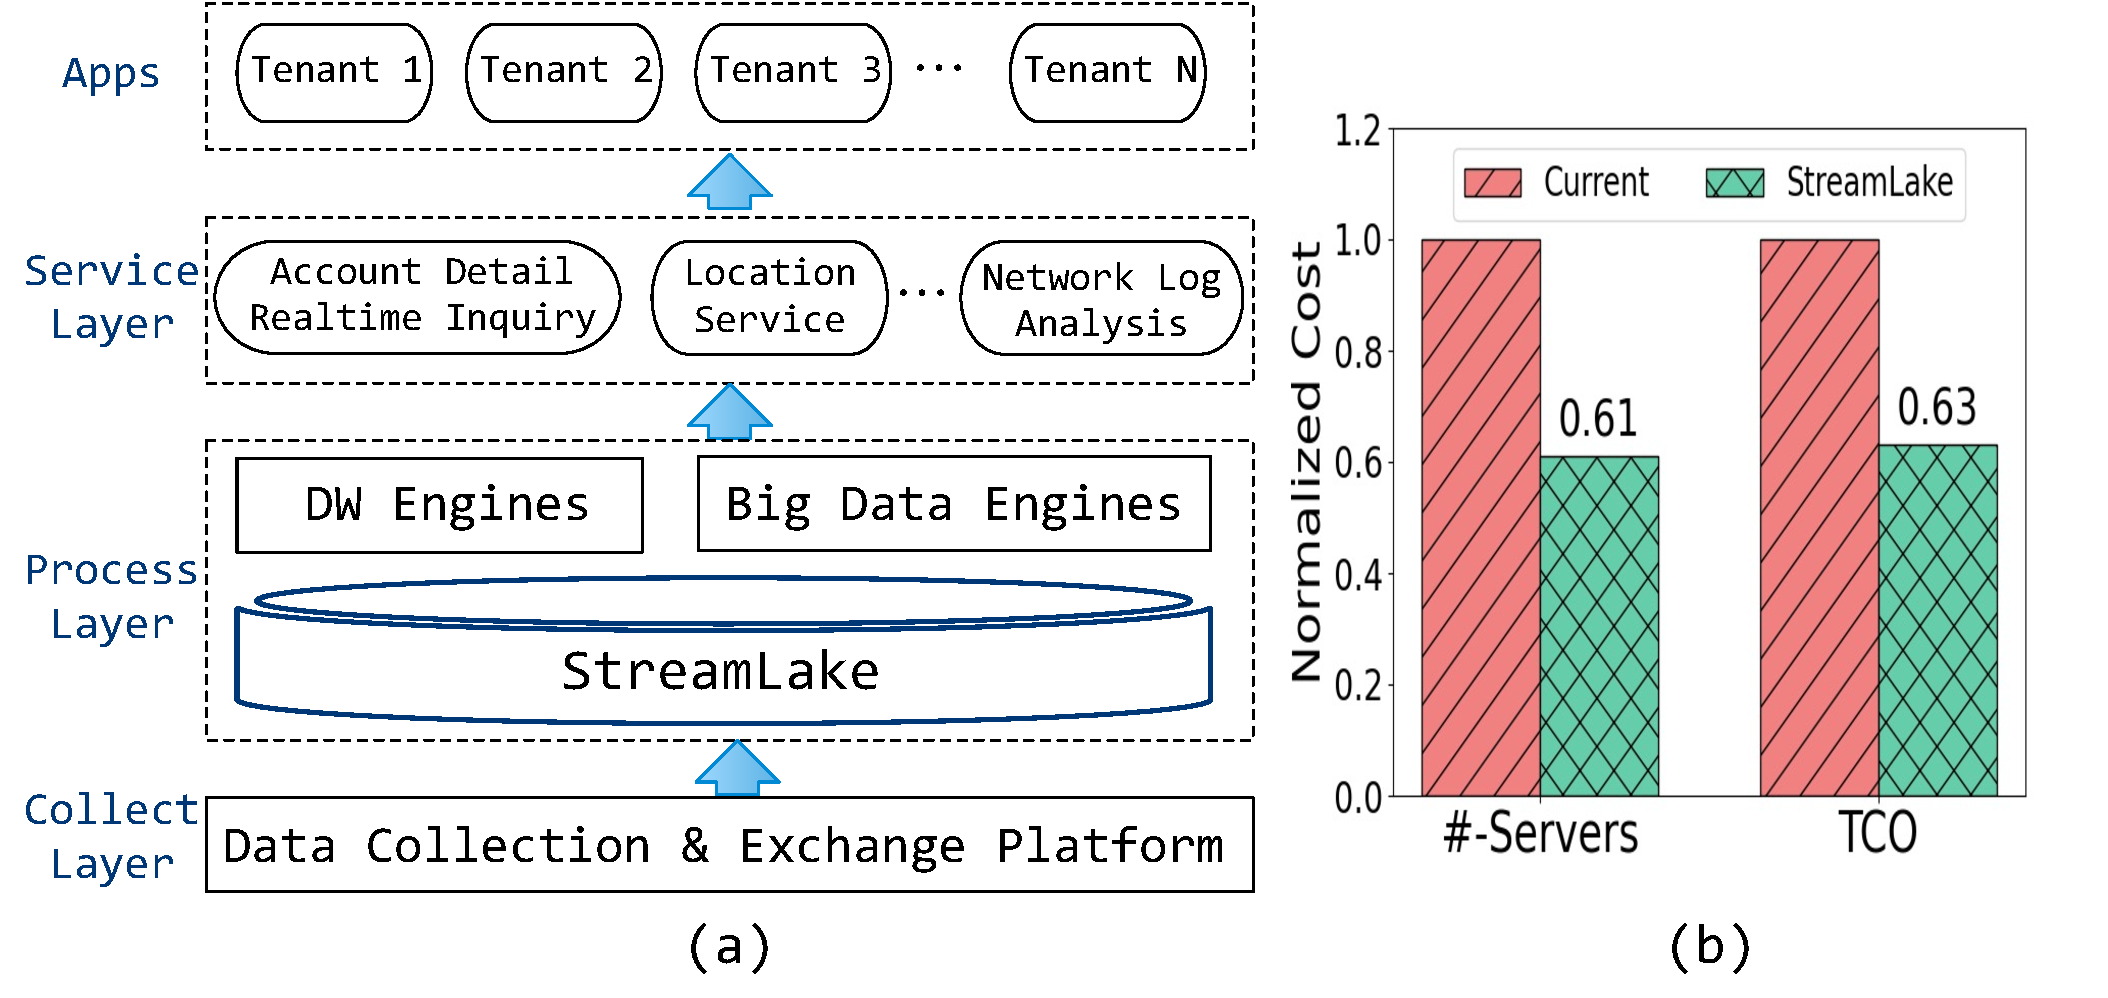
\includegraphics[scale=0.25]{figures/mobile}
	\vspace{-2em}
	\caption{China Mobile Use Case.}
	\label{fig:mobile}
	\vspace{-2.2em}
\end{figure}

\noindent \textbf{Store layer} is responsible for data persistence, which consists of SSD and HDD data storage pools, a high-speed data exchange and interworking bus as well as multiple types of storage semantic abstractions (including block, file, stream, table, etc.).


(1) The data storage pools comprised of SSD and HDD offer reliable management of stored data. The physical storage space on the disks in the storage cluster is divided into slices, which are then organized as logical units across disks in  various servers to ensure data redundancy and load balancing. The storage pools also implement storage space features such as garbage collection, data reconstruction, snapshot, clone, write-once-read-many mechanism, thin provision, etc. 

%The data storage pools comprised of SSD and HDD offer reliable management of stored data. The physical storage space on the disks in the storage cluster is divided into slices, which are then organized as logical units across various servers and disks to ensure data redundancy and load balancing. Additionally, the storage pools incorporate a range of storage space features such as garbage collection, data reconstruction, snapshot, clone, WORM, and thin provisioning.


(2) The data exchange and interworking bus~\cite{huawei} offers high-speed data transfer and interworking of different storage abstractions.Its advanced features include support for Remote Direct Memory Access (RDMA), which bypasses the CPU and L1 cache to accelerate data transfer speeds. Additionally, the bus leverages intelligent stripe aggregation, I/O priority scheduling, etc., to optimize data transfer and processing.
All nodes are interconnected by the data bus to enable high  Input/Output Operations per Second (IOPS), large bandwidth and low latency data exchanges. Furthermore, the bus supports the interworking of different storage abstractions, allowing for the sharing and  access of a single data piece by different interfaces, which eliminates the need for data migration and significantly saves storage space.

(3) The storage abstractions such as block and file  implement access interfaces to the underlying storage in different semantics. We introduce two new abstractions, stream object and table object, to manage messaging streams and tabular data efficiently. 
Their implementation will be discussed in Section~\ref{sec:datagen}.


\noindent \textbf{Data service layer} provides a rich set of features to enable efficient data management at enterprise scale. For instance, the tiering service offers static and dynamic data migration and eviction between the SSD and HDD storage pools based on tiering policies, which saves the storage cost a lot. The replication service provides periodical replications to remote sites for backup and recovery. 

Particularly, to further enhance the capabilities of the layer, we have extended it to include specialized services and optimizations for log message processing operations, which include the \sys  services (Section~\ref{sec:dataeva}) to support real-time streaming and lakehouse functionality, and \brain (Section~\ref{sec:lakebrain}) to improve the resource utilization and query efficiency.
 The elastic serverless function engine can be regarded as a lightweight computation platform to serve the above components.


%To further enhance the capabilities of the Data Service Layer, we have extended it to include specialized services and optimizations for log message processing operations. These include the StreamLake services and LakeBrain optimization, which are elaborated in Sections 5 and 6 of our report.

%To support near-data processing of the StreamLake services, we have introduced a new component called the Elastic Serverless Function Engine. Its design and functionality are discussed in detail in Section 5.3.
 
\begin{figure}[!t]
	\centering
	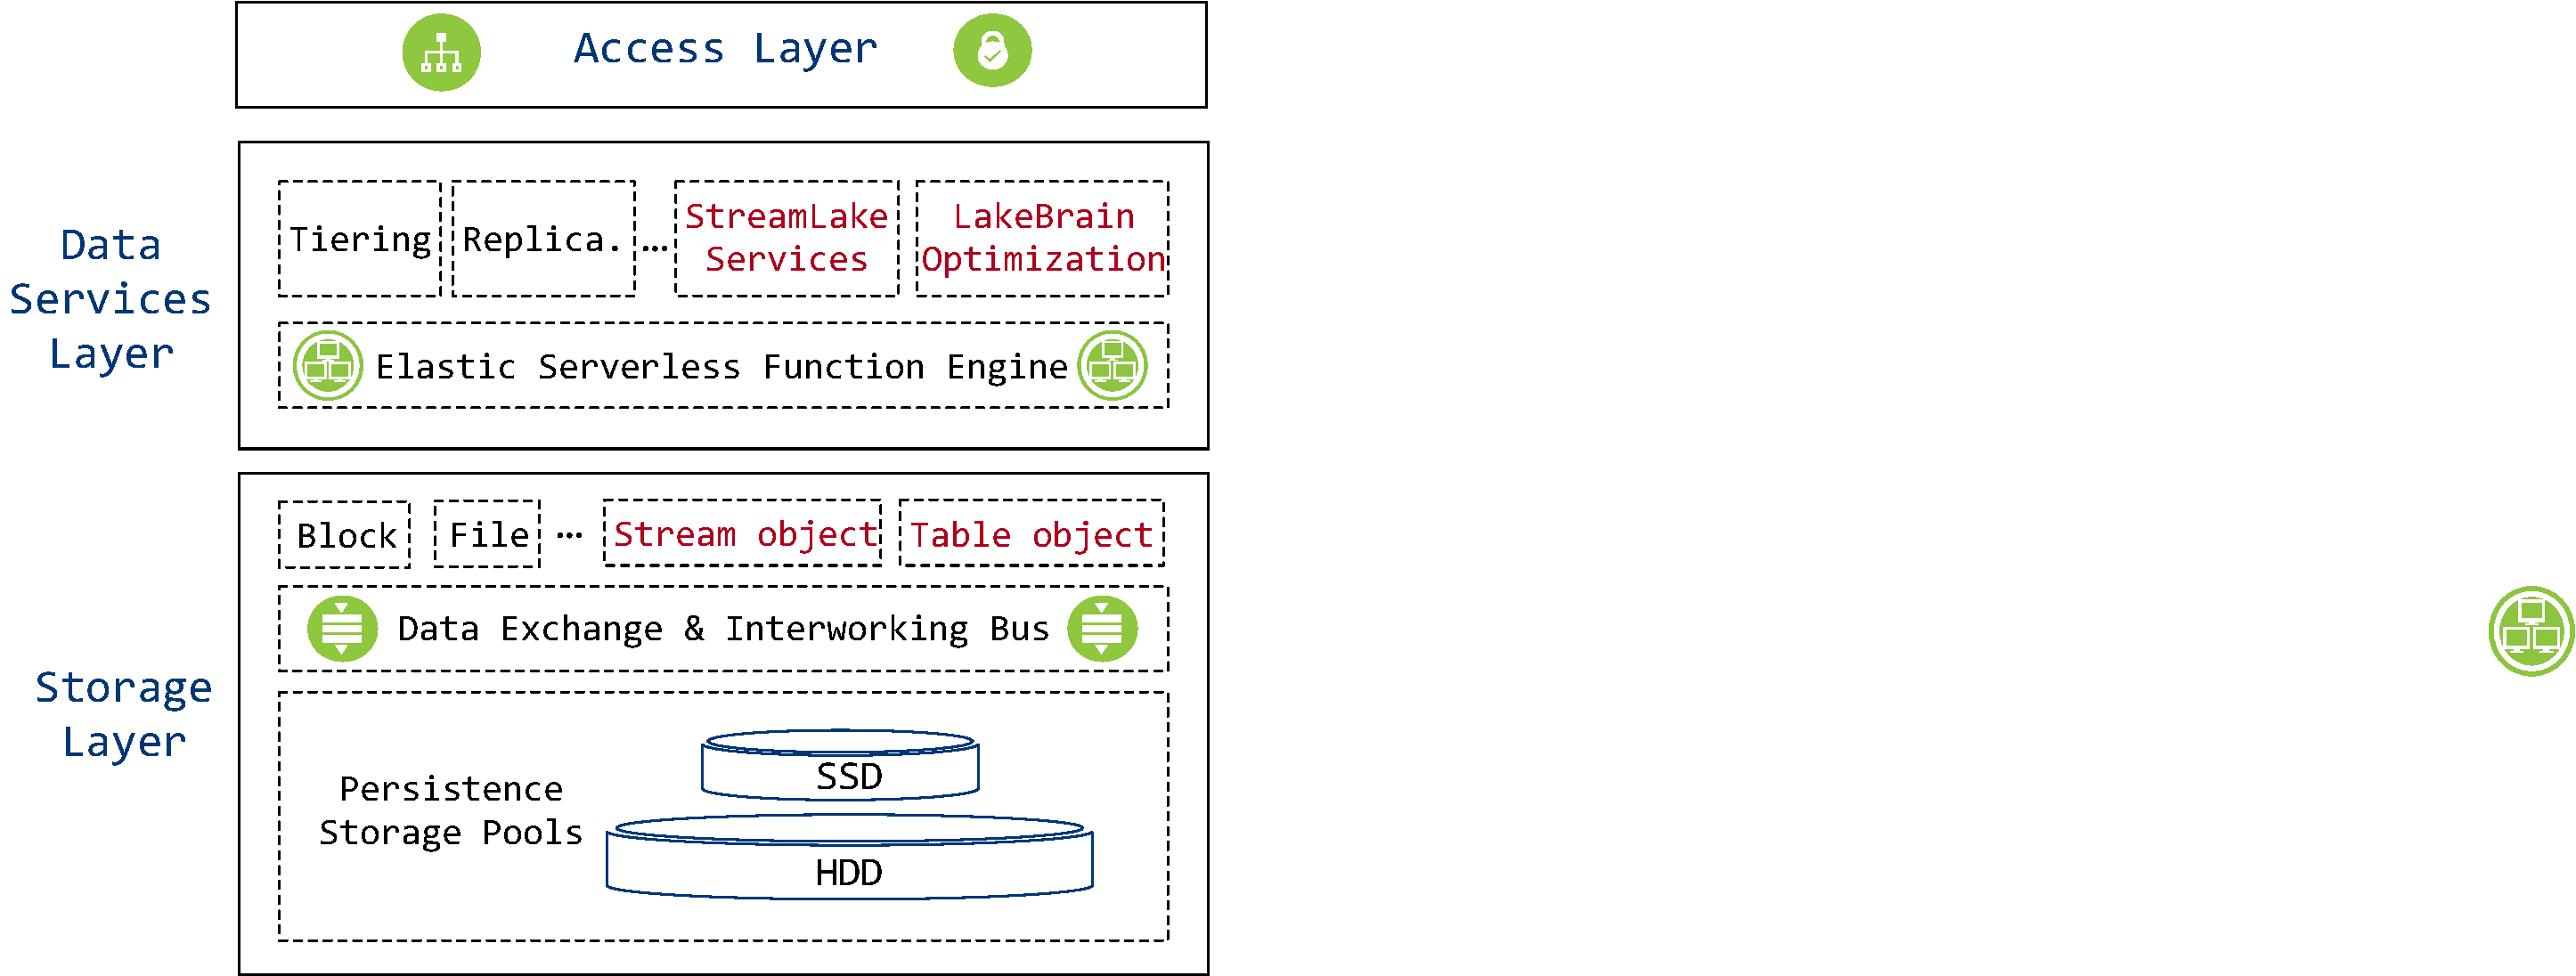
\includegraphics[scale=0.33]{figures/archi}
	\vspace{-1em}
	\caption{\sys Storage Architecture.}
	\label{fig:archi}
	\vspace{-2em}
\end{figure}

\noindent \textbf{Data access layer} implements storage access protocols to handle user requests. It supports a block service via standard iSCSI access, NAS services via NFS and SMB protocols as well as an object service via S3 protocol, etc.
The new StreamLake services utilize the OceanStor distributed Parallel Client (DPC) which is a universal protocol-agnostic client providing shorter but superfast IO path. 
 %The new StreamLake services utilize the OceanStor distributed Parallel Client (DPC), a universal protocol-agnostic client that provides a shorter but super-fast IO path.
The Access Layer also plays a crucial role in managing authentication and access control lists, which ensure that only valid user requests are translated into internal requests for further processing, so as to achieve  the security and integrity.
 
 

 
 
 
%!TEX root = ../main.tex
\section{STREAM AND TABLE STORAGE OBJECT} 
~\label{sec:datagen}

In this section, we introduce the stream object and table object, purpose-built storage abstractions designed for efficient storage and access of stream and table data in the storage layer.


\subsection{Stream Object}~\label{subsec:streamobject}

The stream object is a storage abstraction in the store layer that efficiently supports key-value message streaming at scale. It stores a partition of key-value pairs for continuous message streams, organized as a collection of data slices. Each slice can contain up to 256 records as depicted in Figure~\ref{fig:write}. Incoming message records are appended  to a specific slice in a stream object based on its topic, key, and offset.

\noindent \textbf{Stream objects operations.} The stream object operates similarly to the block and file storage abstractions, providing read and write functionality for stream storage. Figure~\ref{fig:streamobject} outlines key operations supported by the stream object, including creating and destroying a stream object with  functions \texttt{CreateServerStreamObject} (line 1-3) and \texttt{DestroyServerStreamObject} (line 4-5) respectively. The \texttt{$^*$option} field (line 2) sets storage configurations, such as data redundancy methods (replicate or erasure code) and I/O quotas, so as to ensure enterprise-level reliability and performance. The assigned \texttt{objectId} (line 3) serves as a unique identifier for operating the stream object. The \texttt{AppendServerStreamObject} function appends incoming records  to the stream object and returns the starting offset of the appended records. The \texttt{ReadServerStreamObject} function reads the stream object starting from a specified offset, with control conditions such as the length of the read specified in the \texttt{readCtrl} field. 
Since the message service is designed to support real-time streaming, it is set to respond  all subsequent messages unless specified  limits by the user.
\texttt{IO\_CONTENT\_S} (line 8 and 14) is a data structure that provides non-blocking I/O by using buffers to enhance the performance of both writing and reading operations.


\begin{figure}[!t]
	\centering
	\hspace{2.5em}
	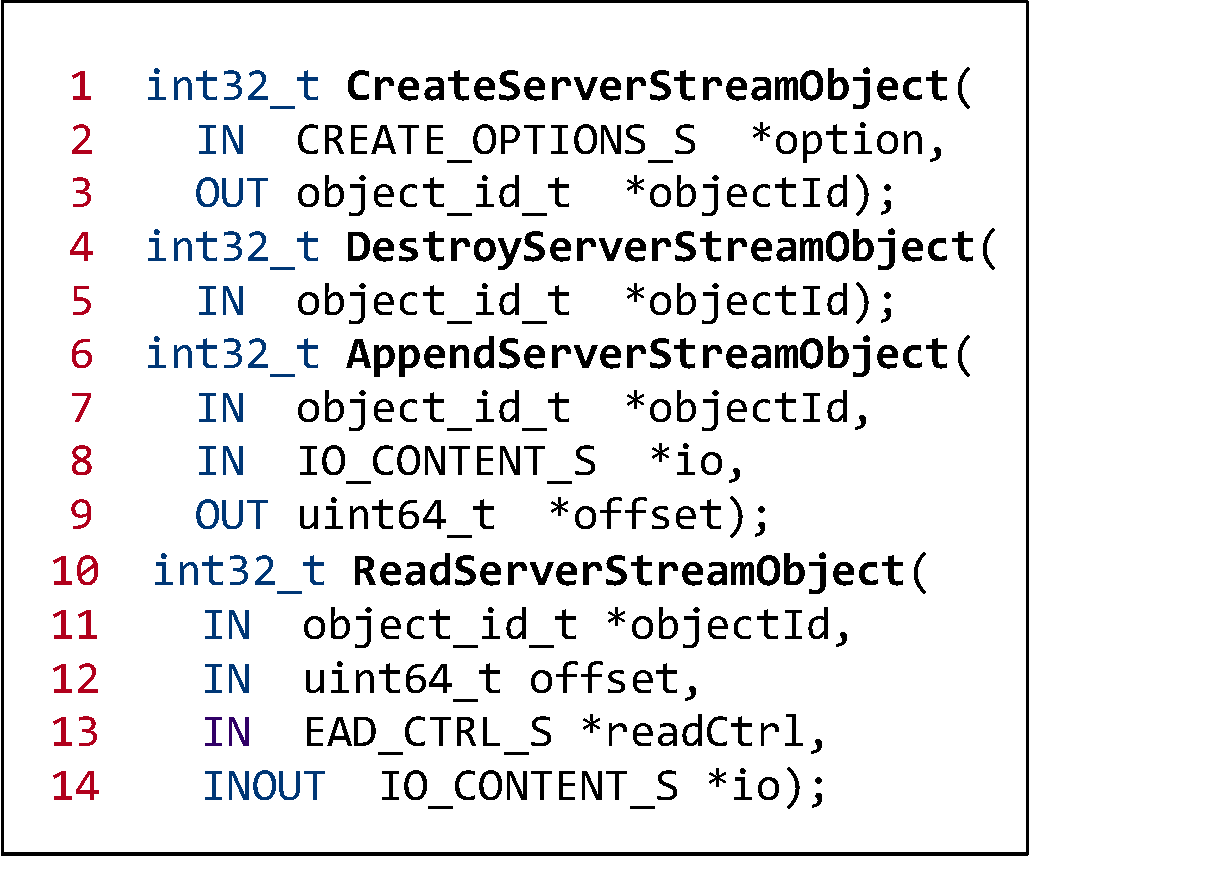
\includegraphics[scale=0.35]{figures/streamobject}
	\vspace{-1em}
	\caption{Stream Object Operations.}
	\label{fig:streamobject}
	\vspace{-2em}
\end{figure}



\noindent \textbf{Write stream messages.} We discuss how to write messages into \sys and endure enterprise-level load-balanced and redundant persistence for the stream objects, which is achieved on the basis of SSD and HDD storage pools.  As shown in Figure~\ref{fig:write}, the messages are first   assigned to stream object slices based on topics, keys, and offsets (Figure~\ref{fig:write}-a,b,c). Then, a distributed hash table is leveraged to ensure even data distribution for load-balance storage (Figure~\ref{fig:write}-d). Specifically, data slices will be distributed evenly to 4096 logical shards, each of which has the storage space managed by persistence logs (PLog, Figure~\ref{fig:write}-e). Each PLog unit is a collection of persistence services in OceanStor~\cite{huawei} that controls a fixed amount of storage space on multiple disks and provides 128 MB of addresses per shard. When a message is received, the PLog unit replicates it to multiple disks for redundancy (Figure~\ref{fig:write}-f). We use  key-value databases to serve as indexes for PLogs for fast record lookup.


\begin{figure}[htbp]	
	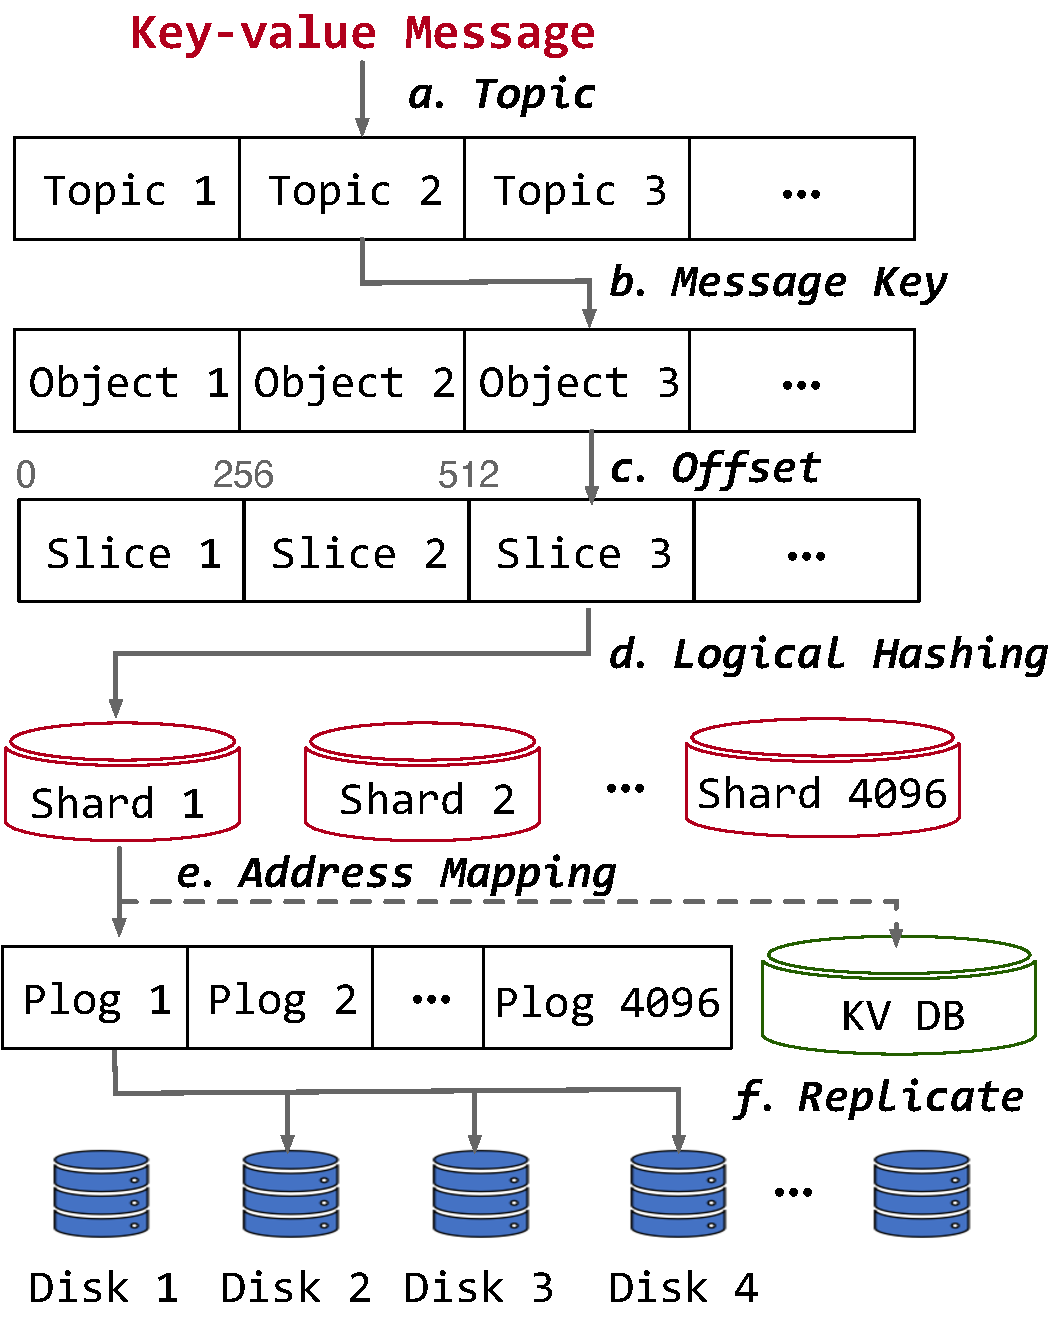
\includegraphics[scale=0.3]{figures/write}
	\centering
	\vspace{-1em}
	\caption{Write Message to \sys.}
	\label{fig:write}
	\vspace{-1em}
\end{figure}


\subsection{Table Object}~\label{subsec:tableobject}
We also extend the storage object layer in \sys to support operations over tables for more effective data storage and management, like the lakehouse systems~\cite{iceberg,hudi,delta}. The table storage uses an open lakehouse format with putting catalog in KV store  for faster metadata access. The table abstraction is logically defined by a directory of data and metadata files, as shown an example  in Figure~\ref{fig:tableobject}.

\noindent \textbf{\texttt{Data} directory.} Table objects are stored in Parquet files of the \texttt{data} directory. In this example, the table is partitioned based on the date column, so the data objects are separated into different sub-directories by the location. Each sub-directory name represents its partition range. The data objects in each Parquet file are organized as row-groups and stored in a columnar format for efficient data analysis. Footers in the Parquet files contain statistics to support data skipping within the file.




\noindent \textbf{\texttt{Metadata} directory}  keeps track of the file paths of the table, table schema,  and transaction commits etc., which are organized into three levels: commit, snapshot, and catalog, as shown in Figure~\ref{fig:tableobject}-(b, c, d).

 \noindent \underline{\textit{Commits}} are \texttt{Arvo} files that contain file-level metadata and statistics such as file paths, record counts, and value ranges for the data objects. Each data insert, update, and delete operation will generate a new commit file to record changes of the data object files.


\noindent \underline{\textit{Snapshots}} are index files that index  valid commit files for a specified time period. These snapshots document commit statistics such as current files, row count and added/removed files/rows as data operation logs. Along with commits, snapshots provide snapshot-level isolation to support optimistic concurrency control. Readers can access the data by reading from the valid commit files, while changes made by a writer will not be visible to readers until they are committed and recorded in a snapshot. This allows for multiple readers and one writer to access the data simultaneously without the need for locks. 

Snapshots also monitor the expiration of all commits, making them essential for supporting time travel. Time travel queries allow data to be viewed as it appeared at a specific time. By keeping old commits and snapshots, the table object enables the use of a timestamp to look up the corresponding snapshot and commits, so as to access to historical data.

\noindent \underline{\textit{Catalog}}  describes the table object, including the profile data  such as the table ID, directory paths, schema, snapshot descriptions, modification timestamps, etc. The data and metadata files are stored in the table directory, except for the catalog, which is stored in a distributed key-value engine optimized for RDMA and SCM to ensure fast metadata access. The data and metadata files are converted to PLogs in the underlying storage for redundant persistence as discussed above.



\begin{figure}[htbp]
	
	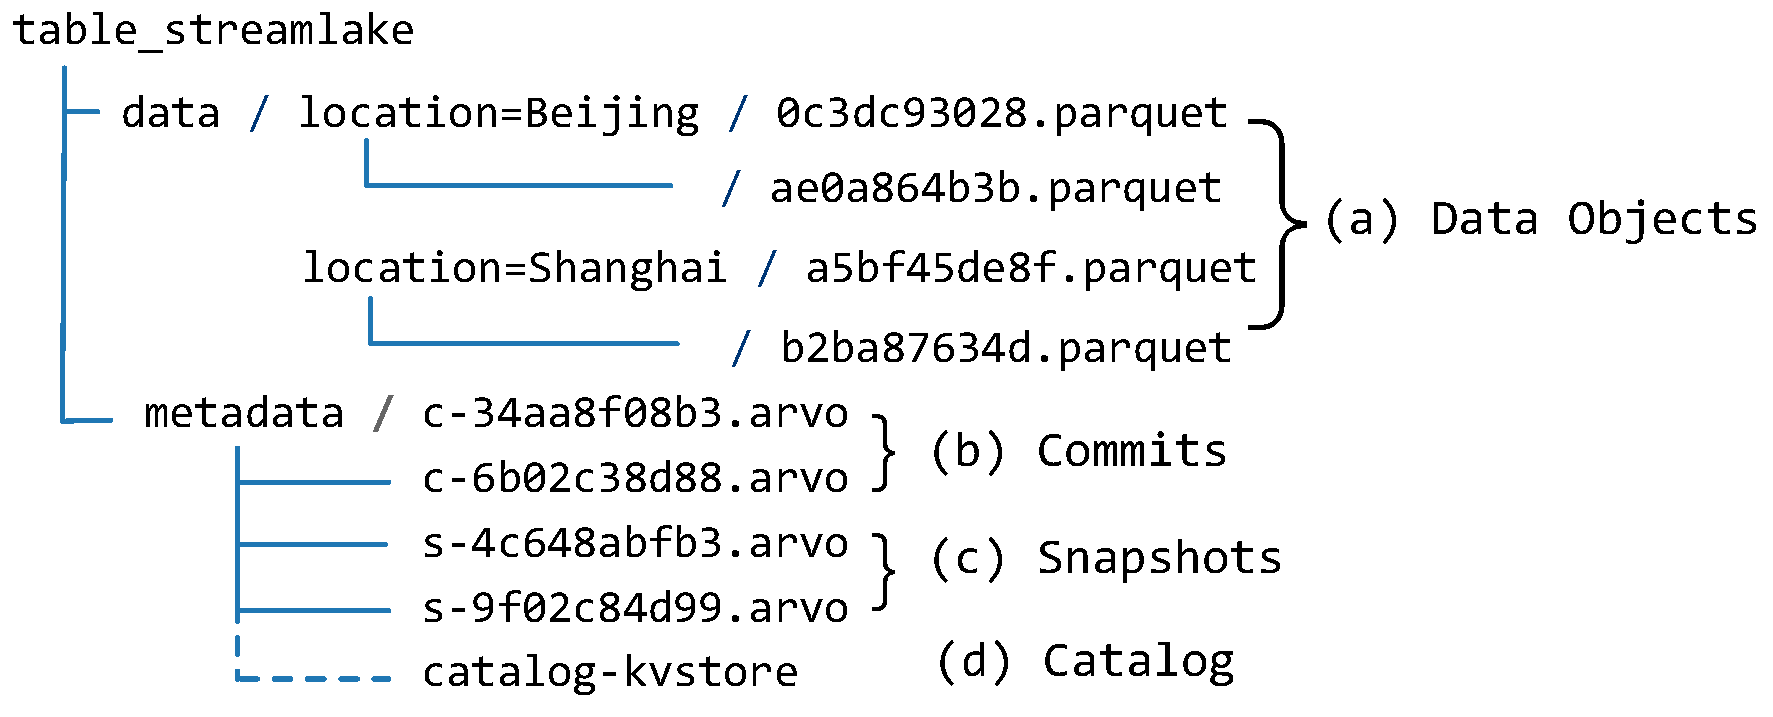
\includegraphics[scale=0.3]{figures/tableobjects}
	\centering
	\vspace{-1em}
	\caption{File Organization of \sys Table Objects.}
	\label{fig:tableobject}
	\vspace{-1em}
\end{figure}



















%!TEX root = ../main.tex
\section{Streamlake Data Processing} 
\label{sec:dataeva}

In this Section, we present the data processing services  in the data layer. Driven by practical application scenarios discussed in Section~\ref{sec:intro}, these services provide a comprehensive, enterprise-level data lake storage solution  to efficiently store and process  log messages at scale. The StreamLake services encompass a stream storage system for message streaming (Section~\ref{subsec:stream}), lakehouse-format read/write capabilities for efficient tabular data processing (Section~\ref{subsec:lakehouse}),  and support for query operator computation pushdown (Section~\ref{subsec:pushdown}).

%\cc{where can we say sth about co-processing?}




\subsection{Message Streaming}~\label{subsec:stream}
We develop a  distributed stream storage engine that facilitates message streaming at large scale. Our engine leverages the stream object storage abstraction to ensure enterprise-level scalability via the disaggregated storage architecture.


\noindent\textbf{Overall architecture of streaming service.} The high-level design of the stream service is shown in Figure~\ref{fig:service}.
 The stream storage system comprises of producers, consumers, stream workers, stream objects, and a stream dispatcher, which work together to provide seamless message streaming. The stream objects are located in the store layer, while stream workers and dispatcher are in the data services layer of \sys.


\begin{figure}[htbp]
	
	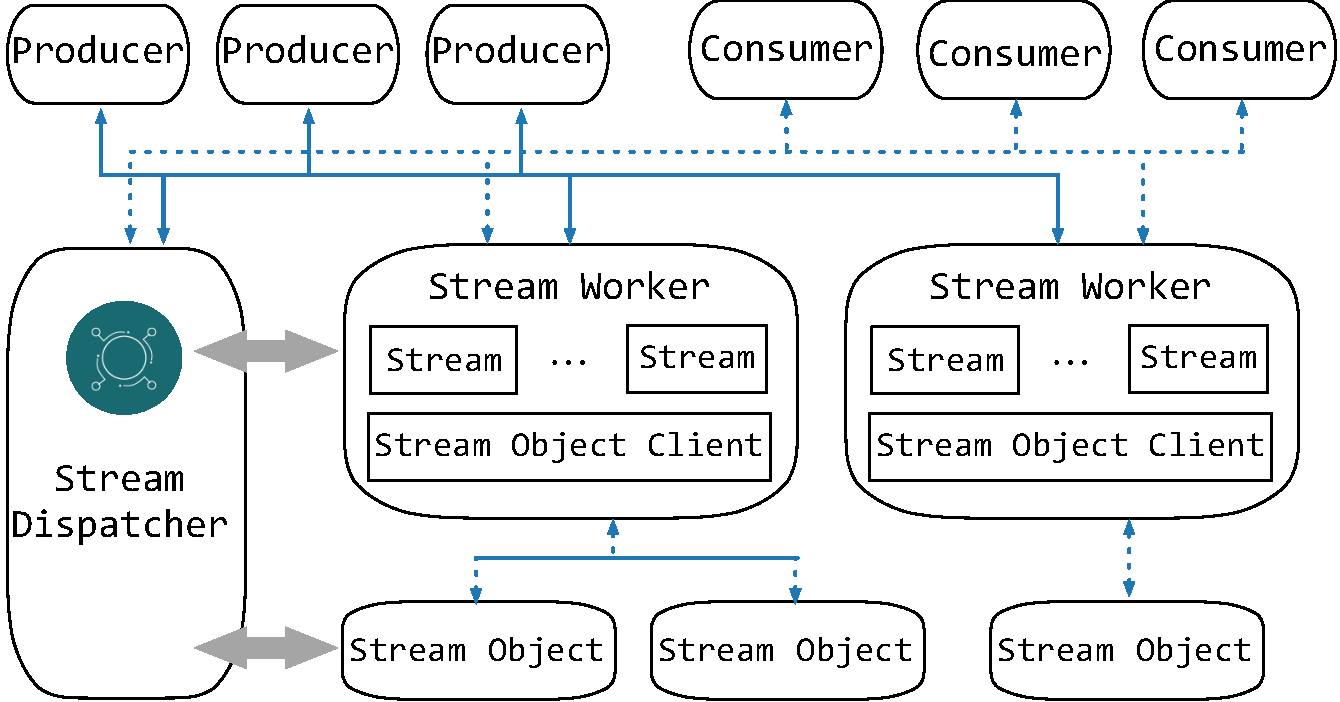
\includegraphics[scale=0.36]{figures/streamservice}
	\centering
	\vspace{-1em}
	\caption{Write Message to \sys.}
	\label{fig:service}
	\vspace{-1em}
\end{figure}

\noindent\underline{\textit{Producers and Consumers.}} Producers are responsible for publishing messages to topics, which are named resources for categorizing streaming messages. Consumers, located downstream, subscribe to these topics to receive and process the published messages. To ensure seamless integration with existing open-source message streaming services used by our customers in production environments, the producer and consumer message APIs are designed to be compatible with the open-source de facto standard. This maximizes connectivity with the ecosystem, allowing users to easily migrate their applications to \sys with minimum costs. Figure~\ref{fig:producer}  demonstrates the process of writing and reading messages using the producer and consumer APIs. In this example, a producer writes a new message ``Hello World'' as a key-value pair to a topic named ``\texttt{topic\_streamlake\_tes}''. The consumer then subscribes to this topic and processes published messages.

\begin{figure}[htbp]
	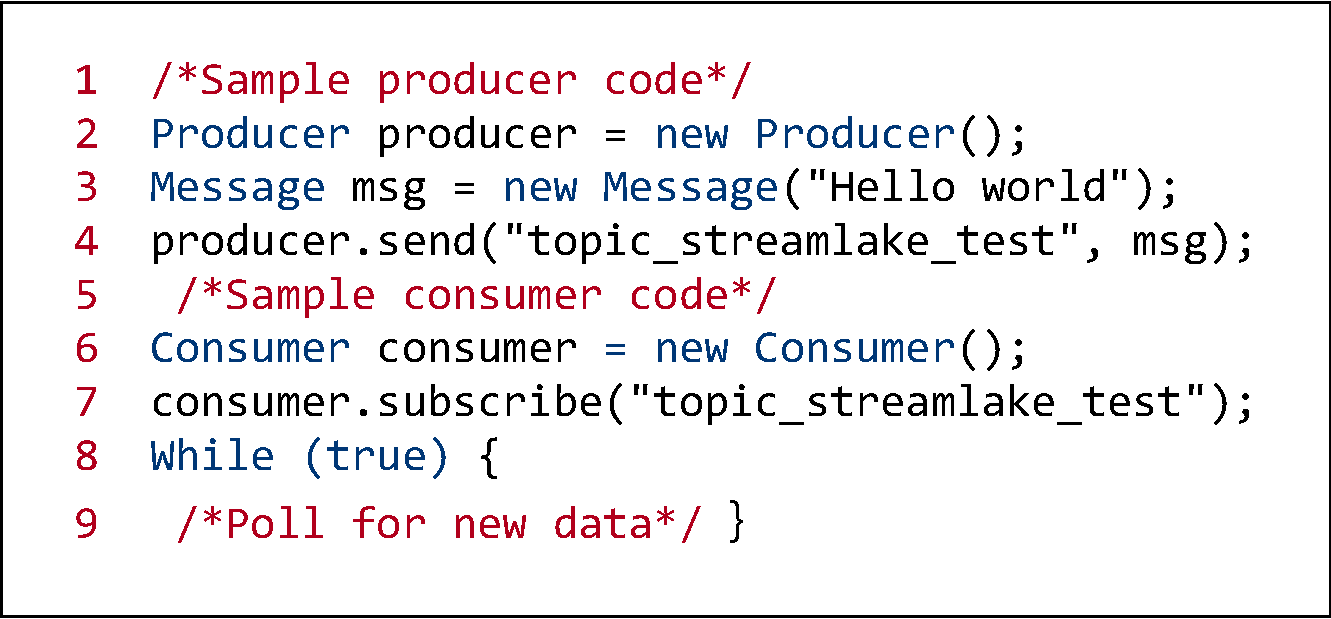
\includegraphics[scale=0.3]{figures/producer}
	\centering
	\vspace{-1em}
	\caption{Sample code of Producer and Consumer.}
	\label{fig:producer}
	\vspace{-1em}
\end{figure}

\noindent\underline{\textit{Stream workers}} work together with stream objects discussed in Section~\ref{subsec:streamobject} to tackle stream processing and message storage. The number of stream workers is determined by configurations and the physical resources allocated to the stream storage. Each stream worker is capable of handling multiple streams and a single stream object client. When a topic is created, streams are added to the stream workers in a round-robin manner to ensure even distribution and workload balancing across the cluster.

Each stream is mapped to a unique stream object in the storage layer, which is a  storage abstraction customized to  key-value message streaming. The stream object offers efficient interfaces and implementations for writing and reading streams from the storage pools. The persistence process is detailed in Figure~\ref{fig:write}.

The task of message delivery is carried out by stream object clients, which monitor the stream objects. These clients unwrap messages from clients, encapsulate them in the stream object data format, and redirect them to the corresponding stream objects via RDMA. To guarantee message delivery, the clients actively monitor the health of the stream objects to which they are connected and regularly exchange critical service data with the dispatcher service. This synchronization process includes reporting the health of the stream object connections and refreshing the stream objects connected to by the client.


\noindent\underline{\textit{Stream dispatcher.}} The stream dispatcher is responsible for managing the metadata and configurations of the messaging service, and directing external/internal requests to the appropriate resources for message  dispatch. The relationships among topics, streams, stream workers, and stream objects are stored as key-value pairs in a fault-tolerant key-value store within the stream dispatcher. When there is  a status change   (\eg a stream worker or topic is added or removed), the metadata  in the key-value store is updated immediately to refresh the topology tracking. This topology tracking aids the stream dispatcher in directing requests for message stream dispatch. When there is a producer or consumer connection request, the stream dispatcher will route the request to the appropriate stream worker based on the associated stream topic, establishing a direct message exchange channel between the producer, the stream worker, and the consumer.

\begin{figure}[htbp]
	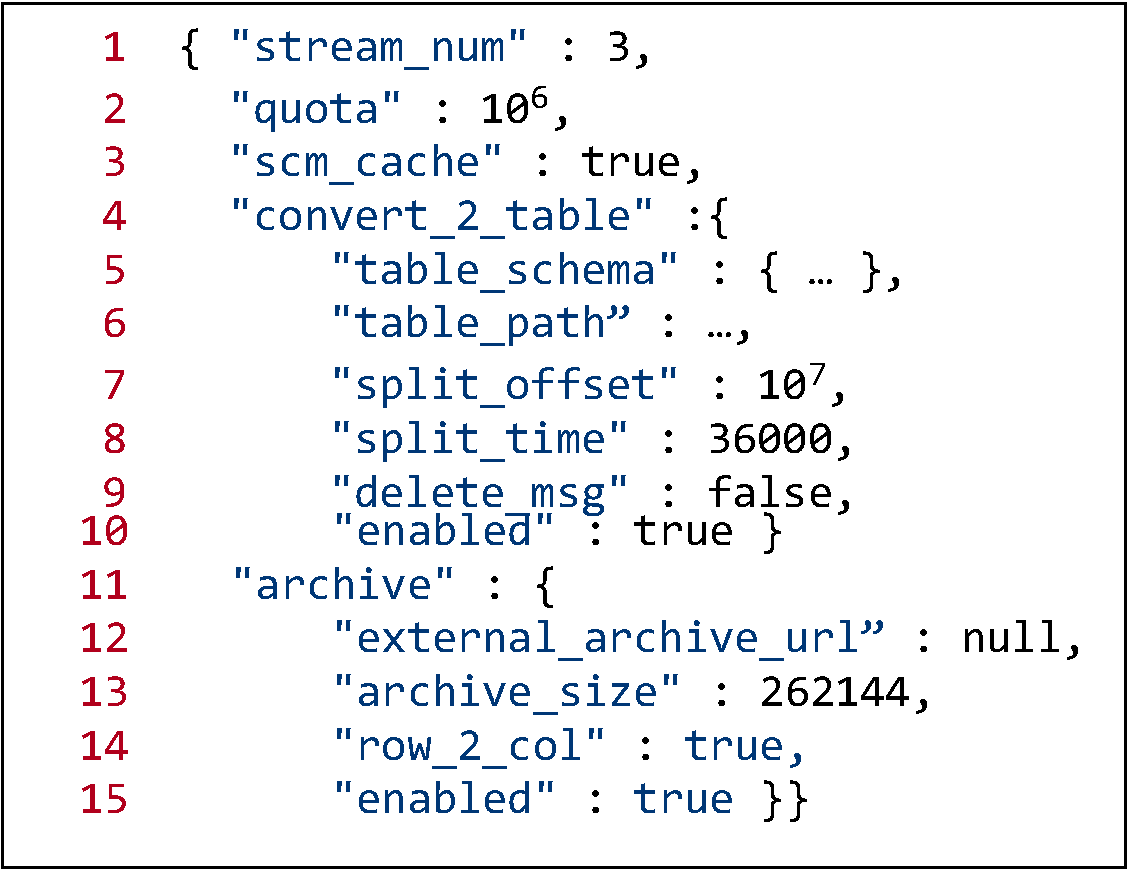
\includegraphics[scale=0.35]{figures/config}
	\centering
	\vspace{-1em}
	\caption{Stream Storage Configuration Example..}
	\label{fig:config}
	\vspace{-1em}
\end{figure}


The stream dispatcher also sets configurations for the messaging service in the unit of topic. An example of  configurations is shown in Figure~\ref{fig:config}.



$\bullet$~\textit{The \texttt{stream\_num} configuration} sets the parallelism of a topic, which should be provided during topic declaration. In the example, three streams are created for the topic and they are evenly distributed among stream workers to process messages in parallel.

$\bullet$~\textit{The \texttt{quota} configuration} sets the maximum processing rate for each stream. In the example, each stream can process up to $10^6$ messages per second.

$\bullet$~\textit{The \texttt{scm\_cache} configuration} enables the use of storage class memory (SCM) caches.

$\bullet$~\textit{The \texttt{convert\_2\_table} configuration} enables the automatic conversion of stream object messages to table object records, and it can also be converted back. When it is set, a background process will apply the \texttt{table\_schema} to convert messages to table object records periodically and save them in \texttt{table\_path}, \ie the table object directory. The conversion is triggered by either an accumulation of $10^7$ messages or the passing of 36000 seconds.  The advantage of this configuration will be illustrated in Section~\ref{subsec:lakehouse}.





$\bullet$~\textit{The \texttt{archive} configuration} automates the archiving of historical data to meet business and regulatory requirements. Data can be stored in the cost-effective \sys archive storage pool or automatically exported to an external storage system specified in the \textit{\texttt{external\_archive\_url} configuration}. The \textit{\texttt{archive\_size} configuration} denotes the data volume in MB that triggers archiving, and the \textit{\texttt{row\_2\_col} configuration} determines whether the data is archived in a columnar format. 

Overall, the \sys stream storage provides guaranteed delivery, efficient transfer, and high elasticity for enterprise use.

\noindent\textbf{Delivery Guarantee:} Our system ensures consistent message delivery through several measures. (1) Data within a stream object is strictly ordered, ensuring that messages are consumed in the order in which they are received. (2) Message writing is idempotent, which means that for network failure, duplicate messages sent by the producer  can be identified.
 (3) Strong data consistency is achieved by eliminating unreliable components like file systems and page caches, and storing data in  stream objects that can tolerant node, network, and disk failures. (4) The system provides exactly-once semantics through the use of a transaction manager and the two-phase commit protocol. This tracks participant actions and ensures that all results in a transaction are visible or invisible at the same time.
 
 %There are two typical scenarios. The first is that a producer writes a batch of messages to multiple streams. All messages are either successfully written or failed. The second scenario is that the application reads the message, processes the message, and writes the message to a new stream and the whole process are either successful or failed.

\noindent\textbf{Efficient Transfer:} Our system implements several mechanisms to efficiently transfer data. First, Stream workers and stream objects are connected through a data bus with RDMA, which reduces the switch overhead in the TCP/IP protocol stack. Second, an I/O aggregation mechanism is used to aggregate small I/O requests and increase throughput. This function can be disabled for latency-sensitive scenarios. Finally, a local cache is implemented at the stream object client to speed up message consumption.

\noindent\textbf{High Scalability:} Our system provides high elasticity by decoupling data storage and data serving to achieve high scalability. The number of stream workers can be adjusted without data migration, and the mapping between stream workers and stream objects can be updated to reflect the changes in a matter of seconds. This allows the message streaming service to easily scale up or down to accommodate changes in service demand.



\subsection{Lakehouse Read and Write}~\label{subsec:lakehouse}

 \sys also provides support for concurrent tabular data reads and writes, similar to  the architecture of lakehouse~\cite{}.
 Besides directly inserting tabular data, we can also get it from the conversion from streaming data.
  In this section, we first  describe the storage conversion from stream messages to tabular records, and then the implementation of key lakehouse operations.
 
 %insert table

\noindent \textbf{Stream-to-table conversion.} This process is performed by a background service and results in the conversion of records in stream objects to table objects, allowing for efficient downstream processing, which is triggered by the \texttt{convert\_2\_table} configuration in Figure~\ref{fig:config}, which include the table schema and time for data freshness in the downstream processing.  The table schema must be specified at the topic declaration, as it determines the expectations for field types and values across all messages. 
 To effectively leverage the storage, users  can choose to just retain messages in crucial topics as stream objects  to support real time applications while converting most stream data to table objects.  The reverse conversion, from table records to stream messages, is also supported for data playback. 
 %As shown in Figure~\ref{exp:fig:case} and Table~\ref{tab:case}, this design provides a good trade-off  between the system cost and latency, which also  helps to decouple the data processing from the business logics.
 This conversion helps to reduce the storage cost because we can just store one copy to achieve both stream and batch processing. Also, this design can reduce unnecessary data movement between the storage and compute clusters for data conversion.




For tabular data processing, our \sys services implement lakehouse read/write operations using a table object and high-performance caches to accelerate concurrent data reads and writes. In the rest of this subsection, we will introduce the implementation of key read/write operations in details.

\noindent \textbf{\texttt{CREATE TABLE:}} This operation begins by registering the table information, such as the schema, path, database, and table name, in the catalog. The \texttt{/data} and \texttt{/metadata} directories are then created under the table path. Then table configurations (schema, partition specification, target file size, etc.) are written to the metadata directory for persistence.



\noindent \textbf{\texttt{INSERT:}} This operation includes the persistence of data and metadata, as well as caching of metadata to the non-volatile memory (NVM), which is introduced to combine small I/O accesses to the underlying storage pools.

\noindent \underline{\textit{(a) Data persistence:}} Records are written directly to the persistent layer as parquet files in the corresponding partition path under the table root directory.


%\cc{There seems should be an emphasize.}

\noindent \underline{\textit{(b) Metadata caching:}} Metadata updates are mostly small I/O operations. 
To avoid generating significant number of small files, we leverage a global write cache to aggregate the metadata updates, which is achieved through the following steps:
(b-1) Each added parquet file generates a commit record containing file-level metadata and descriptions. All new commit records are written to the write cache as key-value pairs when a commit is made.
(b-2) The latest snapshot will be read from the persistence layer to the cache and its commit data will be updated.
(b-3) The snapshot descriptions and version history in the catalog are also read from the persistence layer and  overwritten by adding the latest snapshot description. 

\noindent \underline{\textit{(c) Metadata persistence:}} Metadata in the NVM write cache is asynchronously flushed to the persistent storage pool when the buffer is full. A metadata management process (\texttt{MetaFresher}) transforms the commits and snapshots from key-value pairs to files and writes them to the \texttt{table/metadata} directory.

\begin{figure}[htbp]
	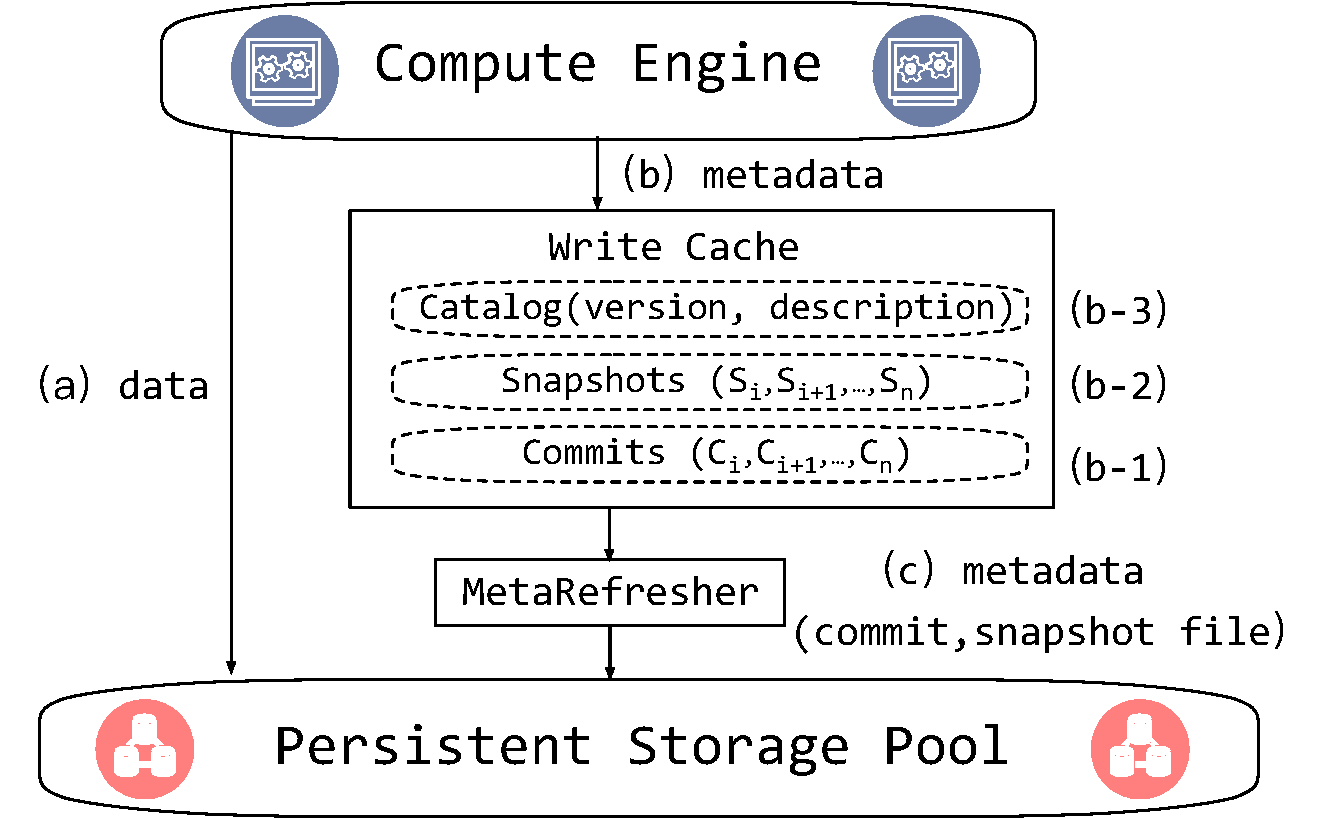
\includegraphics[scale=0.3]{figures/cache}
	\centering
	\vspace{-1em}
	\caption{Write Cache Acceleration in Lakehouse Read/Write.}
	\label{fig:cache}
	\vspace{-1em}
\end{figure}


\noindent \textbf{\texttt{SELECT:}} The select operation first reads the catalog to retrieve the table profile for collecting the list of snapshot files needed for this query, such as the metadata version and snapshot descriptions. Then the corresponding snapshots and commit metadata are read from both the NVM cache and the persistent storage pool to generate the latest complete snapshots and commit metadata. When all the record file addresses are confirmed, data is read from the persistence pool by read tasks.

\noindent \textbf{\texttt{DELETE:}} The delete operation begins with a select operation to find files containing records that match the filtering conditions. There are two cases to consider:
If the filtering conditions match all data in several partitions, only the metadata will be updated, and a new commit version will be generated by eliminating the information of deleted partitions.
If the filtering conditions only match some files, these files will be read, and the data matching the filtering condition will be deleted. Computation pushdowns are applied to process file reads and writes to reduce data transmission to/from the compute engines.


\noindent \textbf{\texttt{UPDATE:}} Similar to the delete operation, update operation also uses a select statement to identify records that match the specified conditions. Optimizations, such as pushdowns, are applied to reduce data movements during the file read and write processes.

\noindent \textbf{\texttt{Drop Table:}} There are two types of drop table operations:
 (1) Drop table soft unregisters the table from the catalog but retains the table's metadata and data in the persistent layer for potential future restoration. To restore a soft-deleted table, a new table can be created and linked to the original table path, effectively registering the deleted table back to the catalog.
(2) Drop table hard  removes both the metadata (files under \texttt{/metadata}) and data (files under \texttt{/data}) of the table and clears the table from the catalog. Note that some of the metadata may have been written to the acceleration cache during the drop table hard operation and will be flushed to the persistent layer asynchronously in the background. The operation to delete the metadata will first clear it from the cache, and then delete it from the disk.

\subsection{Query Operator Computation Push Down}~\label{subsec:pushdown}




In this subsection, we introduce the computation pushdown (similar to S3 Select~\cite{}) to reduce the amount of data transfer between the  storage engine of \sys and the query engines.  Our pushdown method is built on top of an elastic, serverless engine in the data service layer. Here, we choose serverless computing as our execution model because it is lightweight  and flexible, which allows us to quickly start a large number of instances for computation tasks near the data sources, and free the resources as soon as the tasks are completed. The elasticity is important since CPU resources can be scarce during critical data management jobs.

The main components of the serverless function engine are shown in Figure~\ref{fig:serverless}, which include function dispatcher, worker instances, a worker manager, and a function repository. The function dispatcher schedules jobs and manages workflows, and worker instances execute the tasks. The worker manager oversees server resources and the life cycle of worker instances, and the function repository registers and stores function images. These modules work together to support elastic serverless computing.



\begin{figure}[htbp]
	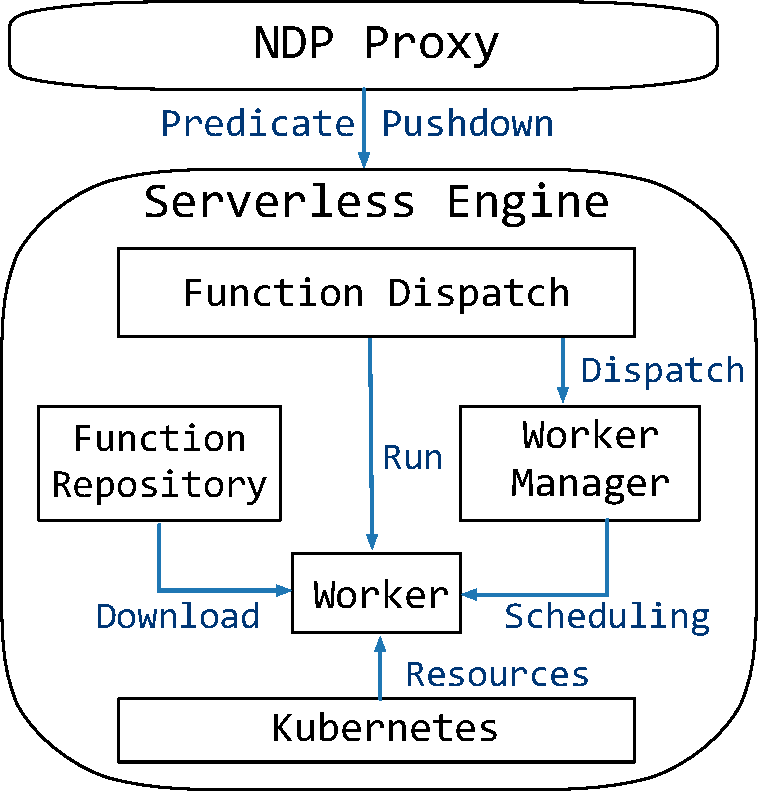
\includegraphics[scale=0.35]{figures/serverless}
	\centering
	\vspace{-1em}
	\caption{Serverless Function Engine.}
	\label{fig:serverless}
	\vspace{-1em}
\end{figure}

To be specific, when a job request is received, the function dispatcher obtains the data location from the storage devices and selects the appropriate storage nodes based on data distribution and available resources. The worker manager is then requested to deploy worker instances to the selected node. The worker instances download the necessary functions from the repository and execute the jobs using data from the storage infrastructure. Upon completion, a callback message is sent to the caller to notify them of the results. To ensure service quality, elastic scaling policies are used to dynamically adjust the number of nodes based on workload. 
For example, a load-balanced method\footnote{not specific} is used to balance scheduling among instances.


To achieve maximum pushdown benefits, three categories of query operators are supported, 

\begin{itemize}

\item \texttt{Projection Pushdown:}  Only selected columns will be returned.

\item \texttt{Filter Pushdown:} Only rows satisfying the filtering conditions will be returned.

\item \texttt{Aggregate  Pushdown:} The results of aggregate functions such as \texttt{Count}, \texttt{MAX} and \texttt{AVG} will be returned.

\end{itemize}

These operators are selected because the size of their output could be significantly smaller than the input, and thereby a large optimization opportunity can be achieved.
These query operators are implemented as separate functions, which are registered and executed in the serverless engine service. The implementation allows for sharing and reuse of the same query operator function by different query engines, as long as its image is registered in the serverless engine.


 %Finally, we build and open sourced plugins [14, 28] for popular big data engines such as Hive, Spark, and Presto [13, 32] to invoke query operator  pushdown. Users can easily install these plugins and speed up critical query processing

To facilitate the pushdown of query operators from the compute layer to the storage cluster in \sys, we have introduced the near data processing (NDP) Proxy and compute engine plugins for popular big data engines such as Hive, Spark, and Presto~\cite{} to invoke query operator  pushdown. 
 During query planning, the optimizer of  query  identifies operators that can be pushed down and sends the information to the NDP Proxy.  Then the NDP Proxy inserts these requests into a queue for traffic control and then sends them to the serverless engine for execution as shown in Figure~\ref{fig:serverless}.
As soon as the query results are ready, the NDP Proxy transfers them back to the compute engine using the high-speed data exchange bus of \sys, so as to ensure efficient data transfer.
Overall,  this process leverages the flexibility and elasticity of serverless computing, which allows for efficient use and release of server resources as required, resulting in better overall performance and resource utilization. 
In addition, inspired by  methods proposed by~\cite{xiangyou, napa}, query operator pushdown can be used together with materialized views as cache to further optimize query performance.  This feature is on the roadmap to add to  \sys. 





%xiangyao yu




















%!TEX root = ../main.tex


%(3) In data lake storage,  it is challenging to perform  optimization like in a database because the computing engine is always decoupled with the storage. Hence, it is critical to consider how to incorporate an optimizer in the storage engine, so as to optimize system performance.


% Third,  we build an intelligent data lake optimizer \brain at the storage-side that focuses on optimizing the data layout in the storage, so as to improve the resource utilization as well as  query performance. Many recent works~\cite{}  have focused on using machine learning techniques to  optimize database systems, including the knob tuner, query optimizer etc. For the data lake system with the disaggregated storage, we think that it is a promising direction to design an optimizer and we conduct the following two attempts. We design a reinforcement learning based automatic compaction module  to decide whether to compact small files considering the system state at a certain system status, so as to \cc{improve the block utilization while keeping the system running smoothly.} We also build a predicate-aware partitioning model that is utilized to judiciously distribute data to storage blocks to reduce the number of blocks to be visited, so as to improve the query efficiency. 

\section{Lakebrain optimization} 
\label{sec:lakebrain}




%\cc{Below is very hard to follow! what is talking about?where is the partition? what is the connection with the above?}


%LakeBrain's design is kept simple for ease of extension and support for different applications. It consists of three components: a statistics collector, the core optimization logic, and an executor. The statistics collector gathers system configurations, environment variables, and workload history, while the core optimization logic employs heuristic rules, probabilistic models, and machine learning algorithms to suggest the best strategy candidates. The executor then deploys the chosen strategy, with its effects being collected as feedback by the statistics collector for future optimization.


%To demonstrate the value of a data lake storage optimizer, we have developed two LakeBrain applications: auto compaction and predicate-aware fine-grained partitioning. These use cases will be explained in detail in the following section.

Optimizing  query processing over large-scale data is significant in data warehouse and big data systems, as discussed in~\cite{oracle, tere, survey, eltabakh2021not, pandit2015accelerating, armbrust2015spark}. However, for the \sys system with
complicated storage-disaggregated architecture, it is challenging to optimize the query performance and resource usage. The reasons are two-fold. First, it is hard to capture the entire environment about the compute and storage cluster as well as the queries executed by other engines simultaneously. Second, even though all the environment data is available, it is still hard to optimize because of the large search space due to the large number of tunable and interdependent variables~\cite{jindal2021microlearner}.



To address the challenges, we present~\brain, a novel data lake storage optimizer that aims to optimize the  the data layout at the storage-side, so as to improve the resource utilization as well as  query performance.
Unlike query engine optimizers that focus on join order and cardinality estimation~\cite{rtos, deepdb, naru}, \brain aims to optimize data layout in storage, which is key to improve both query performance and storage resource utilization in a storage-disaggregated design. In this Section, we mainly focus on two cases, $i.e.,$ automatic compacting small files  and judiciously partitioning tables to improve the resource utilization improve the query performance.
Next, we will illustrate the above aspects in detail.

\subsection{Automatic Compaction}~\label{subsec:compaction}
In a streaming application scenario, data ingestion and transactions often result in numerous small files, leading to low query performance on merge-on-read (MOR) tables. 
A typical method is to compact files statically using rule-based methods such as setting a time window or a data size threshold~\cite{iceberg,hudi}.
In this part, \brain  designs the automatic compaction to combine these small files into fewer and larger ones, so as to  improve the block utilization  as well as query performance.

The block utilization at a certain state $t$ is defined by $\frac{\sum_{i=1}^{n}f_t^i}{K \times  \sum_{i=1}^{n}\lceil \frac{f_t^i}{K}\rceil}$, where $n_t$ denotes the number of files at the state, $f_t^i$ denotes the size of each file and $K$ is the block size.
 As streaming data is continuously ingested,  we are likely to frequently determine whether to merge small files.
  However, considering a certain state in the system, we cannot simply  compact files when the block utilization is low because both compaction and data ingestion require commits, which may have conflicts, leading to compaction failure or ingestion slow down. On top of that, compaction consumes relatively large amount of computing resource. 
  
   Moreover,  at each state, a number of system parameters \cc{($e.g.,$ file ingestion speed, target file size, etc any more???) } will influence the system, and the action ($i.e.,$ whether to merge files) does not purely influence current system situation, but also future states.
   
    That is, compaction is not a \cc{XX action, and its influence will appear in the future.}

Therefore, we propose a reinforcement learning framework that can well capture the relationship between system parameters of each state and the long-term benefit (considering the future system states) of conducting the compaction or not. 
To be specific, as shown in  Figure~\ref{fig:rl}, 

\noindent \underline{\textit{Agent}} can be taken as our automatic compaction module that receives the \texttt{reward} (resource utilization) and \texttt{state} (system parameters) from the \texttt{environment} (the storage system). Then it updates the policy network ($e.g.,$ DQN~\cite{}) to guide whether to conduct the compaction operation so as to maximize the long-term reward.

\noindent \underline{\textit{State}} denotes the current state of the storage system, described by \cc{many} features, for example, among which \cc{XX} are significant ones closely  related to the compaction problem. These features will be encoded as the input of the policy network.

\noindent \underline{\textit{Reward}}  reflects whether the compaction  has a positive or negative impact on the system and the extent of the impact. Specifically, if the compaction succeeds, the reward is  computed by the improvement of the block utilization. If it fails, the reward is the minus of the number of partitions that participant this compaction.

\noindent \underline{\textit{Action}} denotes whether we conduct the compaction at each state, which is the output of the policy network. If we decide to compact, we will \cc{XXXX}.

Overall, the training process is that given each state in the system, when acting the compaction or files are keeping ingested, the state will change and we can observe the reward provided by the environment. This repeats until the model converges. For inference, as the streaming data comes continuously, we can trigger the trained RL model every few moments to determine whether to  compact the files.

%As discussed above, file compaction aims to find the optimal strategy for compacting files that can improve query execution time or increased block utilization\footnote{not mentioned above} in storage. To achieve this goal, the optimization process employs two algorithms\footnote{two algorithms or steps?}: particle swarm optimization (PSO)\footnote{is there a citation? } and reinforcement learning (RL).

%PSO is used to search for the global optimum, a population-based method that doesn't require assumptions about the relationship between tunable parameters and query performance. The goal is to obtain an approximately optimal solution within a limited time.  \cc{Not clear!! We should say what is the entire problem, and why and how to split it into two steps.}


%\cc{Also not clear!! We should introduce what is the problem and the optimization goal that fit the paradigm of RL. Then define the critical components of RL and illustrate that.} RL secondly finds a more sophisticated policy based on the states of the data lake environment. The optimization process involves considering a set of discrete compaction configurations within the action space. Since the state space is continuous, a function approximation method is preferred. The stability of the training process is critical due to the high degree of variability in query performance in a distributed environment, so proximal policy optimization (PPO) is applied.

\begin{figure}[htbp]
	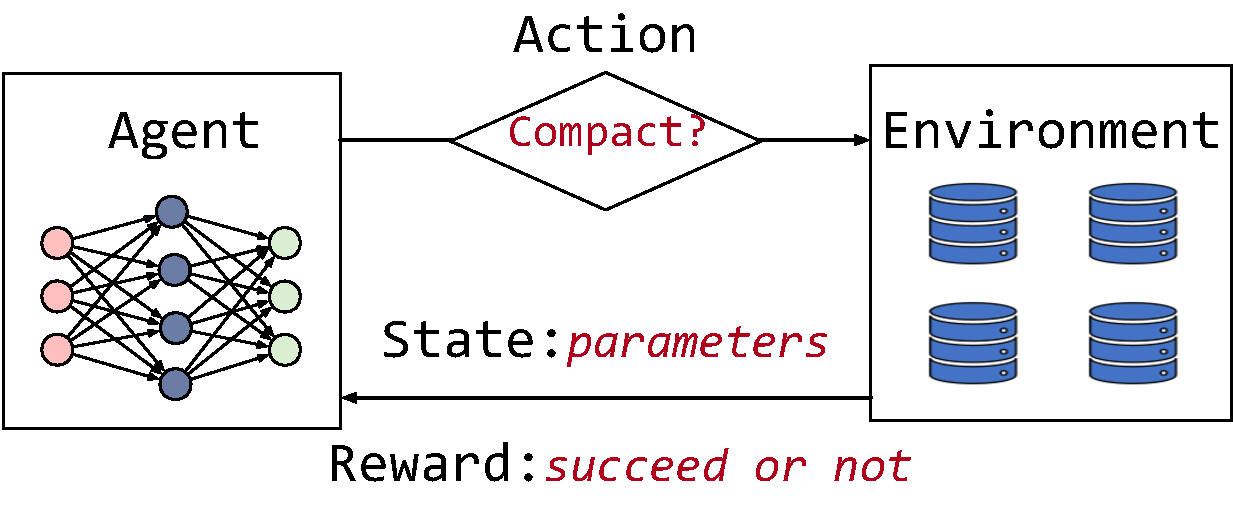
\includegraphics[scale=0.38]{figures/rl}
	\centering
	\vspace{-1em}
	\caption{Automatic Compaction using RL.}
	\label{fig:rl}
	\vspace{-1em}
\end{figure}

%A deep neural network (DNN) is used to approximate the policy and the value function, with a shared feature backbone network that covers both global and local characteristics of the states. The output from the feature network is processed by two fully connected networks to compute the policy output and the action value. The actor and critic are alternatively updated after collecting new trajectories using the latest policy during training.

%Once a desired result is obtained, the numerical output of the compaction strategy is translated into actionable operations by the data lake connector for a specific data lake engine, facilitating the optimization process.






\subsection{Predicate-aware Partitioning}~\label{subsec:partition}


With the data volume increasing, we  have to partition the data into different storage blocks such that the query efficiency can be much improved. In practice, users always select a single (or multiple) column as the partition key,  apply   a hash function to the values of the key, and then distribute the data to different blocks based on the partition values. This method is sub-optimal $w.r.t.$ the latency because it may lead to imbalanced data distribution. \brain  designs predicate-aware  method to partition the data in a fine-grained way such that given a query, the \cc{number of blocks or tuples?} to be assessed is minimized, and thus the efficiency is improved.


\begin{figure}[htbp]
	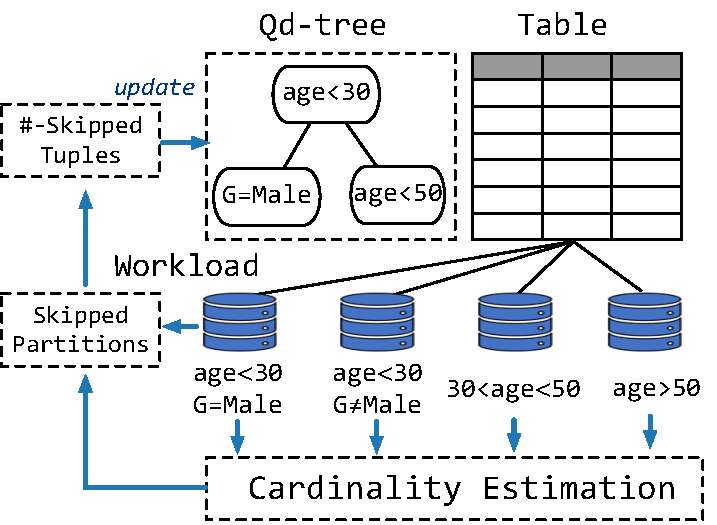
\includegraphics[scale=0.6]{figures/partition}
	\centering
	\vspace{-1em}
	\caption{Predicate-aware Partitioning.}
	\label{fig:partition}
	\vspace{-1em}
\end{figure}


 Specifically, our partition method is based on the query-tree framework~\cite{qdtree}, and additionally leverage the machine learning based cardinality estimation method for optimizing the query tree, so as to find a fine-grained data partition with high query efficiency. 
As shown in Figure~\ref{fig:partition}, given a table $T$ and a query workload $W$ consisting of the pushdown predicates, we will build a query tree, similar to a decision tree where each inner node denotes a predicate in the form of (attribute, operator, literal), where operator includes $\{\leq, \geq, <, >, =, IN\}$. Each leaf node refers to a partition such that when executing $W$, we can skip as many tuples as possible. For example, the leftmost partition contains tuples satisfying $\texttt{age}<30$ \texttt{and} $\texttt{G=Male}$. Given $W$ and the partitions, we can compute how many partitions that we can skip. But in order to compute the number of skipped tuples, we have to know the cardinality of each partition. We can either directly compute the cardinality, or sample for estimation, which is time-consuming or not accurate enough. Hence, we can use AI-driven cardinality estimation methods~\cite{face, e2e, naru, deepdb} to estimate the cardinality accurately and efficiently via learning the data distribution. In practice, we use the sum-product network~\cite{deepdb} as the estimator. 
%Optimizing data partitioning~\footnote{* we should first say what is the data partition problem (does the previous section mention it?)} involves assigning records to storage blocks in the most efficient manner possible, thereby reducing the number of blocks accessed during queries. Our partitioning approach is based on the query-tree framework [43], and utilizes a sum-product network (SPN) probabilistic model [19, 26, 31] to model the distribution of the data in LakeBrain. This is done in order to ensure fast inference speed and avoid repeatedly scanning the datasets.



%The query-tree framework creates a tree-based partitioning strategy using pushdown predicates. Each leaf node represents a partition, and its column ranges are derived from the pushdown predicates used to split its parent nodes.
 %By using probabilistic models to characterize the dataset, we can identify the most suitable partitioning policy. The probabilistic model-based cardinality estimation, as demonstrated in Figure 11, is used to estimate the number of records in each partition, \cc{How?? query-driven or data-driven? both cases should have queries to test} instead of scanning the original data, thereby saving a significant amount of time. This greatly improves the speed of the partitioning optimization algorithm, making it suitable for large-scale systems.

%Additionally, probabilistic models allow us to represent a sequence of datasets with a series of probabilistic models that have a fixed structure but varying parameters. This is achieved by representing a sequence of datasets as a series of multi-dimensional vectors, each representing the learnable variables in the probabilistic model with a fixed length, i.e. a time series. We can then use time series prediction methods to predict future probabilistic models, and use these predictions to estimate the number of records in a partition during partitioning optimization\cc{like a magic}.




%To implement the optimized data layout, we introduce a partitioning mechanism that saves data in fine-grained partitions based on the partitioning strategy. Additionally, we have implemented an evaluator that skips irrelevant partitions by checking the overlap between pushdown predicates and the column ranges in each partition. For numerical columns, the range can be represented as lower and upper bounds, which are well-handled by many data formats. For categorical columns, we either record its range or its complement using "IN" or "NOT IN" predicates. The effectiveness of this predicate-aware partitioning approach is evaluated in section 7.2, where the test results show exceptional performance.

%!TEX root = ../main.tex
\section{Experiment} 
\label{sec:exp}

\subsection{Experimental Settings}


\noindent \textbf{Our Experimental Scenario.} To showcase the effectiveness of the \sys framework, we employ a real-world use case simplified from the case in Section~\ref{sec:intro}.   A mobile financial  company collaborates with China Mobile to collect and analyze its app usage data. The company aims to understand its  usage patterns to prevent frauds and enhance its product experience. 
China Mobile provides this analytic service through an end-to-end big data processing pipeline, which includes several jobs such as data collection, normalization, labeling, and querying, as depicted in Figure~\ref{exp:fig:case}.
We compare  \sys framework with their current solution to build a  pipeline that can facilitate business analysis.

\noindent \underline{\textit{(a) Collection:}}  The network carrier collects mobile app data packets in  data centers and transfers them to a centralized storage pool.


 \begin{figure*}[htbp]
	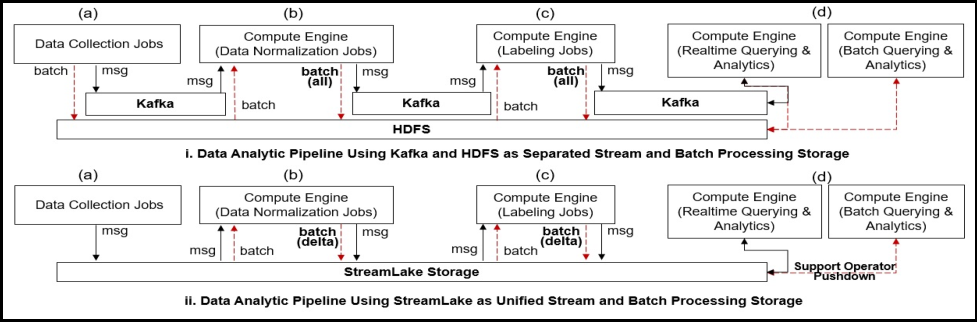
\includegraphics[scale=0.95]{figures/case}
	\centering
	\vspace{-1em}
	\caption{Data Analytic Pipelines for a  Real-world Use Case.}
	\label{exp:fig:case}
	\vspace{-1em}
\end{figure*}
\noindent \underline{\textit{(b) Normalization:}} At the  storage pool, the data packets are normalized as records in a unified schema. Data is validated to ensure accuracy and quality. Sensitive data is shielded to protect  privacy. 

\noindent \underline{\textit{(c) Labeling:}} Labels from knowledge bases are added, so as to classify the records and identify useful insights.

\noindent \underline{\textit{(d) Query:}} After the normalization and labeling  are completed,   records are inserted into tables and  available for query engines. To perform analyses, the app company employs secure API calls to query the data. Figure~\ref{exp:fig:sql} illustrates an example SQL query that counts the daily active users (DAU) in different provinces.% More complicated analysis, like hidden Markov and Gaussian Mixture Models, can also be applied to draw user profiles and identify abnormal activities.

To support both \cc{full} data and real-time analyses, the network carrier builds two data flows in the pipeline. One  processes full data in batch every two hours and the other processes stream messages constantly to deliver time-sensitive logs such as new logins, payments and password modifications. This ensures that the network carrier can effectively analyze both historical data and real-time events to make  accurate and timely decisions.

 \begin{figure}[htbp]
	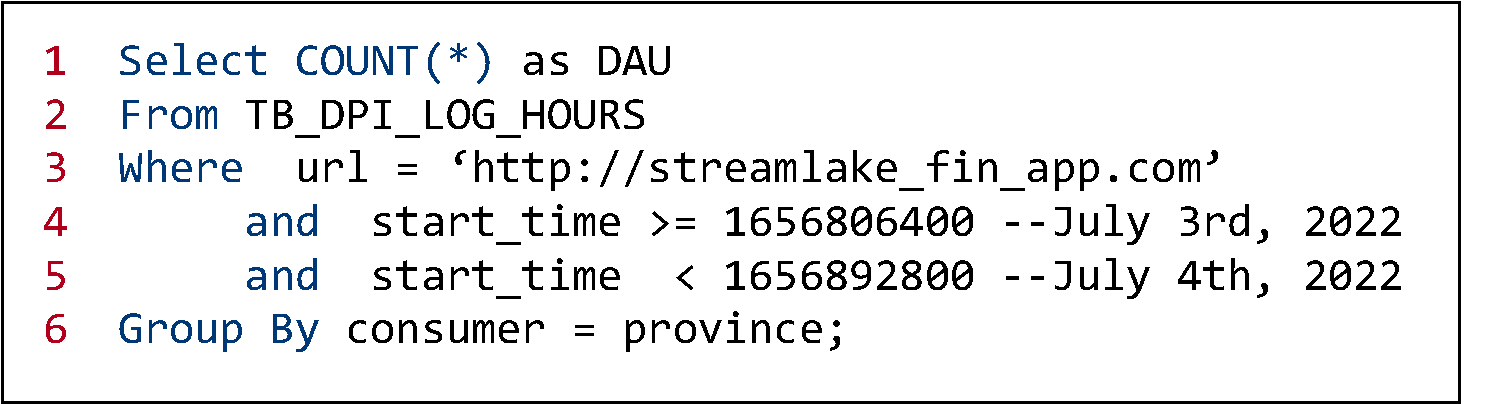
\includegraphics[scale=0.33]{figures/sql}
	\centering
	\vspace{-1.3em}
	\caption{Query Example of Computing DAU.}
	\label{exp:fig:sql}
	\vspace{-2em}
\end{figure}

\noindent \textbf{Settings.} This use case is evaluated in a  cluster using different sizes of input data packets and the results are compared with open-source storage solution Hadoop Distributed File System (\hdfs)~\cite{hdfs} and \kafka~\cite{kafka}. The reason of why we choose the two storage systems is that in reality, China Mobile has been using them for many years, which have shown stable and good performance. Hence, it is  reasonable to directly compare with the systems that our customer (China Mobile) is using. Also, in practice, many of our customers also use HDFS and Kafka to cope with similar application scenarios.


%\cc{For above, do we need more justification? like why hdfs and kafka fit? or common sense?}
%These two storage systems are chosen because of their popularity in real world and are relatively easy to provide context to illustrate the usage of StreamLake.


 
  To be specific, the cluster consists of 3 nodes, each with 24  2.30 GHz cores and 256 GB RAM. The cluster is configured as a 3-node \sys when we measure it.  While running the open-source solution, it is configured to host a 3-node \hdfs storage and a 3-node \kafka cluster simultaneously. The number of input data packets varies: 10 million, 50 million, 100 million, 500 million, and 1 billion packets. Each packet has an average size of 1.2 KB, resulting in corresponding data volumes of 12 GB, 60 GB, 120 GB, 600 GB, and 1.2 TB, respectively.

Overall, Figure~\ref{exp:fig:case} shows the data processing process.  \kafka and \hdfs serve as independent stream storage and batch storage respectively to pass data across collection, normalization, labeling and query jobs.
 As a typical ETL practice, a new copy of all data is written to \hdfs and \kafka after each job. In case  failing accidentally, a job can read its input data to reproduce the results.
 
 

 
  In our solution, \sys serves as a unified stream and batch processing storage. 
  We replace \kafka and \hdfs with \sys, which handles the message streaming and data storage. 
  Only minimal changes are made to the compute engines, so the business logic remains unchanged. 
  As \sys supports time travel, only updated rows are written to the storage. When a job needs to re-run, it can use time travel to retrieve its input data.  During the query jobs, for example, the three filters in the \texttt{WHERE} clause and the \texttt{COUNT} aggregate in Figure~\ref{exp:fig:sql} are pushed down to compute in \sys, so as to  accelerate the query.










\begin{table*}[ht]
	\begin{tabular}{|c|c|c|c|c|c|c|}
		\hline
		&  \#-Data Packet & 10,000,000 & 50,000,000 & 100,000,000 & 500,000,000 & 1,000,000,000 \\ \hline
		\multirow{3}{*}{Storage Space Usage (GB)}                  & \sys              & 34         & 166        & 329         & 1,659       & 3,289         \\ \cline{2-7} 
		& \hdfs + \kafka            & 145        & 729        & 1451        & 6,901       & 13,816        \\ \cline{2-7} 
		& Ratio (HK/S)         & 4.33       & 4.38       & 4.40        & 4.16        & 4.20          \\ \hline
		\multirow{3}{*}{Stream Processing Speed (Messages/Second)} & \sys              & 301,522    & 417,303    & 518,065     & 530,077     & 546,987       \\ \cline{2-7} 
		& \kafka             & 302,611    & 413,613    & 527,826     & 531,021     & 539,893       \\ \cline{2-7} 
		& Ratio (K/S)         & 1.00       & 0.99       & 1.02        & 1.00        & 0.99          \\ \hline
		\multirow{3}{*}{Batch Processing Total Time (Second)}      & \sys             & 259        & 664        & 1173        & 4868        & 9646          \\ \cline{2-7} 
		& \hdfs              & 212        & 795        & 1548        & 7535        & 14771         \\ \cline{2-7} 
		& Ratio (H/S)         & 0.82       & 1.19       & 1.32        & 1.55        & 1.53          \\ \hline
	\end{tabular}
	\caption{\sys v.s. \hdfs and \kafka.}\label{tab:case}
	\vspace{-2.5em}
\end{table*}


\subsection{Overall Comparison}

Table~\ref{tab:case} shows the results. The numbers of input data packets are in the top row. The storage usage and processing time for \sys (S), \hdfs (H), \kafka (K) are in the following rows.  The ``Ratio'' represents that the ratio between \hdfs(\kafka) and \sys with respect to the storage usage or time. 
Note that HK denotes the sum of the storage usage in  \hdfs and \kafka.

The experiment demonstrates that \sys significantly improves the total storage cost and the batch processing time. The storage cost in the \hdfs and \kafka  is 4 times as much as \sys. The reason is that in \hdfs and \kafka, full data is written into the storage when each ETL job is finished, which is a common practice to support downstream jobs restart after unexpected failures. As a result, six copies of full data are written into the storage. 
While for our \sys, we save 75\%  storage cost by saving one copy of full data plus updates in each ETL job via the stream-to-table conversion and lakehouse functionality.

The batch processing speed in \sys is better than \hdfs when the workload is 50 million records or more.  As the workload grows,  \sys is 50\% faster than \hdfs when the workloads are 500 million and 1 billion records because we use the \brain optimizer and  write cache to improve the efficiency.
 On the other hand, \sys may not be the best choice for small workloads. When the workload is 10 million records, \sys is 20\% slower than \hdfs as it performs extra metadata management.
%the advantages of skipping irrelevant partitions and query operation pushdown become significant.
The message stream processing speed in \sys is competitive to \kafka. \sys and \kafka process about 300 thousand messages per second when the workload is 10 million records. Both systems scale to process about 500 thousand messages per second when the workloads are 100 million and more. 


\begin{figure*}
	\centering
	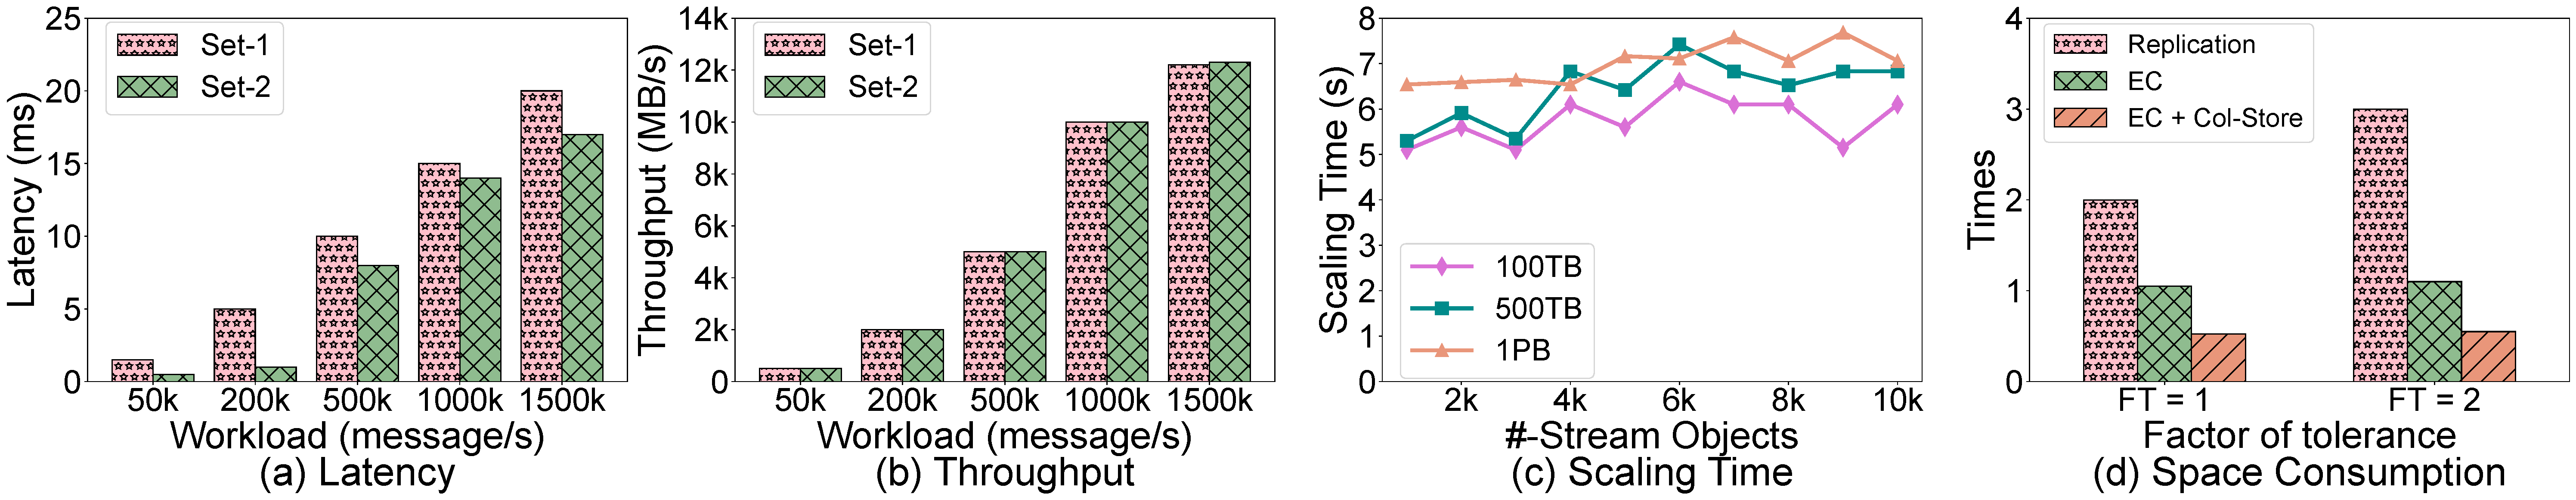
\includegraphics[width=0.92\textwidth]{figures/streamengine}
	\vspace{-1em}
	\caption{Evaluation of Message Streaming.}
	\label{fig:streamengine}
	\vspace{-2em}
\end{figure*}



\subsection{Evaluation of Message Streaming}

To quantitively measure the message streaming service as an independent stream storage, we conduct an experiment to evaluate its throughput, latency, elasticity and volume. We select \texttt{OpenMessaging}~\cite{openmessaging} as our benchmark  because it is widely used to compare messaging platforms. A cluster with three nodes is used in this experiment for  ease of reproduction.
 To help better understand the impact of tiering storage, two sets of hardware configurations are tested. In the first set of hardware (\texttt{Set-1}), each node has 10 CPU cores, 128 GB RAM and 800 GB NVMe SSD, 3 PB SAS HDD and all the nodes are connected with 10 Gb ethernet. In the second set of hardware (\texttt{Set-2}), all the configurations are the same except that each node has additional 16 GB persistent memory to serve as an extra cache. Messages are sent from producers to consumers in a fixed size of 1 KB. The data volumes we process are 100 TB, 500 TB and 1 PB respectively. 


Figure~\ref{fig:streamengine} shows the results in terms of  the latency, throughput, scaling time, and space consumption.
As shown in Figure~\ref{fig:streamengine}(b), persist memory reduces the latency as we expect, especially when the workload is 200k messages per second or less.
When it comes to the throughput (Figure~\ref{fig:streamengine}(a)), as the messages to process increase from 50000 per second to 1.5 million per second, the system throughput increases linearly. 
\texttt{Set-1} and \texttt{Set-2} achieve almost the same throughputs, indicating that it does not improve the throughput to add persistent memory as a cache. 
 Figure~\ref{fig:streamengine}(c) shows the high elasticity of the stream storage. The service gracefully scales from 1000 to 10000 partitions in less than 10 seconds. The good scalability  demonstrates a significant advantage of the   disaggregated storage architecture. 
Finally, Figure~\ref{fig:streamengine}(d) compares the space consumption different storage strategies (\texttt{Replication} refers to  saving data in its original format using multiple copies, \texttt{EC} refers to using erasure code to store the data, \texttt{EC+Col-store} refers to first converting the data to columnar format and then applying erasure code). 
The X-axis, $e.g.,$ \texttt{Fault Tolerance(FT)}=1 means that a storage cluster with the redundancy strategies can tolerant one node failure, and no data is lost.
The  Y-axis means  the times of its original data size   using these redundancy strategies.
 Without scarifying the reliability, \sys provides the options (\texttt{EC} and \texttt{EC+Col-store}) to use erasure coding and column-store which can save three to five times of storage cost compared to \texttt{Replication}. 






\begin{figure*}
	\centering
	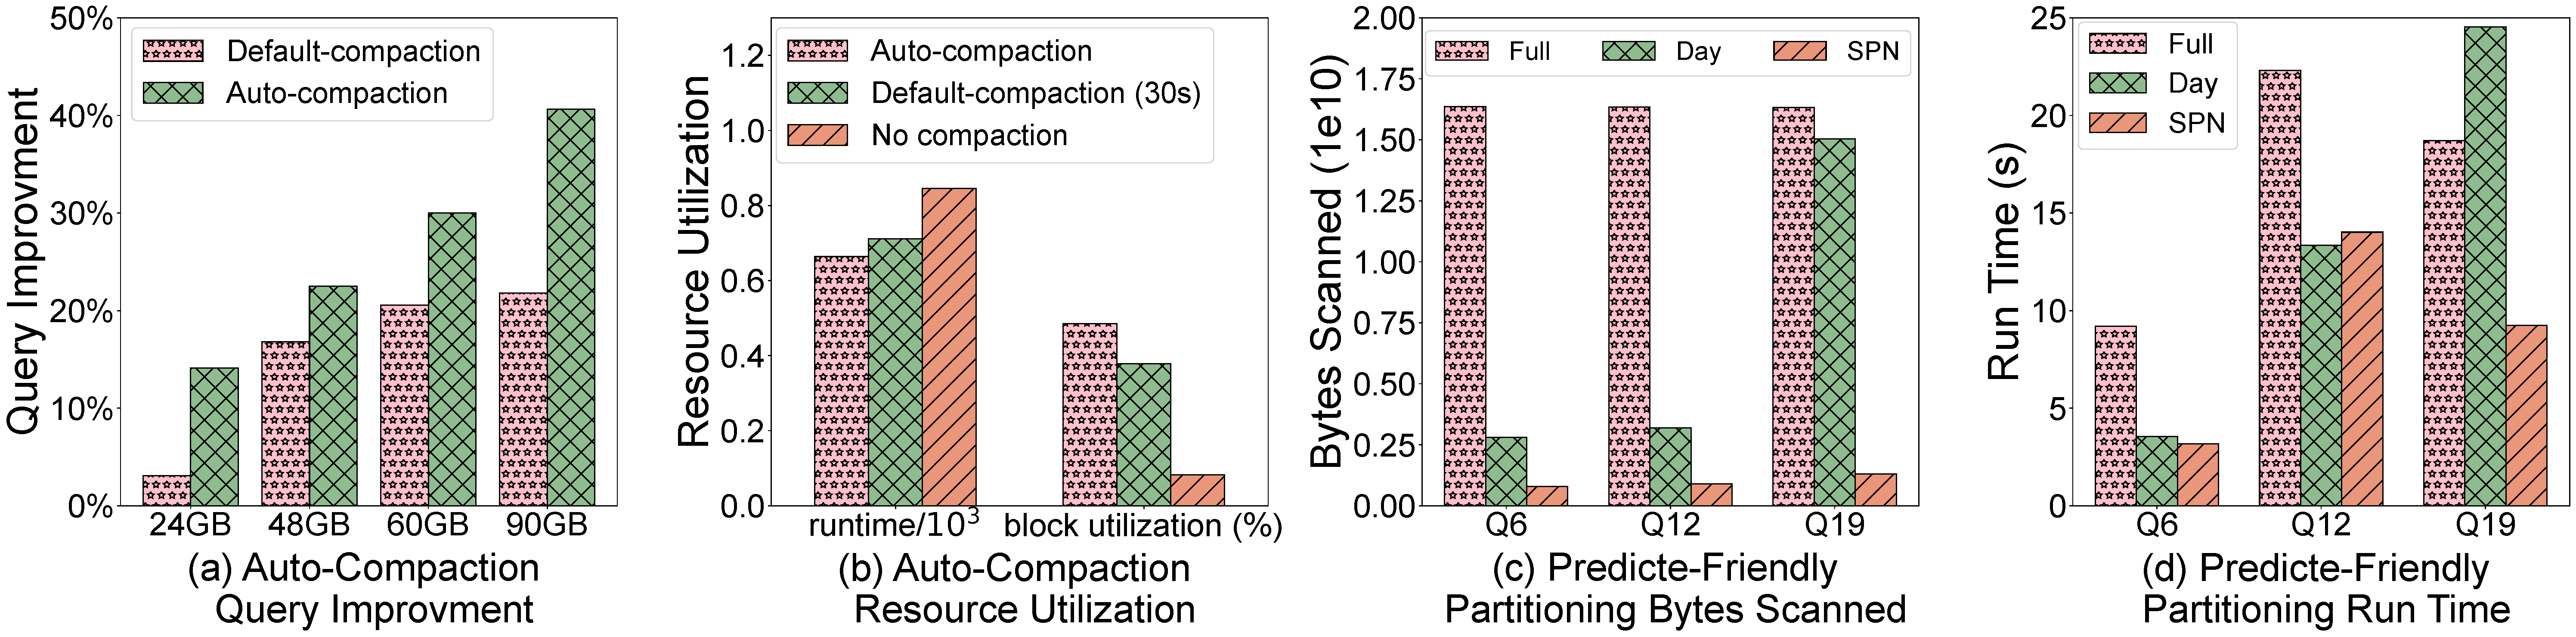
\includegraphics[width=0.9\textwidth]{figures/LakeBrain}
	\vspace{-1em}
	\caption{\cc{LakeBrain Compaction and Partitioning Performance.}}
	\label{fig:lakebrain}
	\vspace{-1em}
\end{figure*}



\subsection{Evaluation of \brain}

In this part, we evaluate the two components in \brain.

 
\noindent \textbf{Auto-Compaction:} To precisely evaluate the effectiveness of our automatic compaction strategy, a \texttt{TPC-H} based test bed is set up to ingest data from the message streaming platform to the data lake storage, during which a compaction strategy is tested.
 We run the experiment with 24 GB to 90 GB data and compare our \texttt{Auto-compaction} in \sys with \texttt{Default-compaction strategy}, $i.e.,$ a static strategy which simply compacts data files in a 30 second interval. 
During the ingestion, multiple rounds of \texttt{TPC-H} queries are executed in parallel  to obtain their end-to-end performance. As shown in Figure~\ref{fig:lakebrain}(a), the results depict how much improvement of  query performance that the compaction strategies can make, compared with the baseline.
 We can observe that the auto-compaction strategy outperforms the static one for all data volumes. As the data volume increases, the advantage becomes more significant because the number of blocks to be visited is reduced.




In addition to the query performance, we also evaluate the block utilization of the auto-compaction. Specifically, we control the file ingestion speed such that we can generate different numbers of files to measure both the run time and the block utilization in different workloads. The run time is evaluated along with the block utilization because an ideal strategy should improve the utilization without scarifying the performance. Similar to above, we deploy three methods: (1) No compaction, (2) The static strategy compacts data files in a 30 second interval, and (3) Auto-compaction. We can observe that the auto-compaction outperforms the static strategy in term of block utilization.  When we deploy the auto-compaction, the system is able to identify good compaction opportunities in which there are many small files and both the file ingestion speed and the block utilization are relatively low. 
File ingestion speed is important because compaction commits will fail if there are file access conflicts. As a comparison, it is hardly to avoid unnecessary or unsuccessful compaction in the static compaction strategy hence its performance is not good. Figure~\ref{fig:lakebrain}(b) shows the results of all three test groups.






\noindent \textbf{Predicate-Aware Partitioning:} We also test the partitioning method on \texttt{TPC-H}  with different scale factors. We train the probabilistic model with 3\% of the data randomly sampled from the \texttt{lineitem} table in a dataset generated with a scale factor of 2. After that, we obtain the optimized partitioning policy with the proposed method and evaluate our system on the full dataset with scale factors of 2, 5, 10 and 100. To evaluate the performance, we compare the resulting bytes skipped for \texttt{lineitem} table with (1) No partition (\texttt{full}). (2) Partition by the day of \texttt{l\_shipdate} (\texttt{day}).  (3) Our  method using sum-product networks~\cite{deepdb}  (\texttt{spn}) as the cardinality estimator.
 We compare the results with partitioning by the day of \texttt{l\_shipdate} considering it appears frequently in the pushdown predicates. The workload includes \texttt{TPC-H} query 6, 12 and 19 which involve \texttt{lineitem} table and include predicates other than \texttt{l\_shipdate}. We skip other \texttt{TPC-H} queries because their performance is  mainly dominated by the joins of multiple tables, which is beyond our purpose.
 
 \cc{Below is not clear enough!}

The results  in Figure~\ref{fig:lakebrain}(c,d) shows that the proposed method obtains non-marginal performance gains in terms of both \cc{bytes scanned} and the runtime. The fine-grained partitioning is superior on the queries in terms of data skipping compared to partitioning by the day of \texttt{l\_shipdate} because the optimized partitioning policy split the data based on other predicates except \texttt{l\_shipdate}. Even though the runtime for the queries is dominated by table joining, the optimized partitioning also demonstrates some improvement for query 6 and query 19, considering we only optimize the partition of the \texttt{lineitem} table. 



\begin{figure}
	\centering
	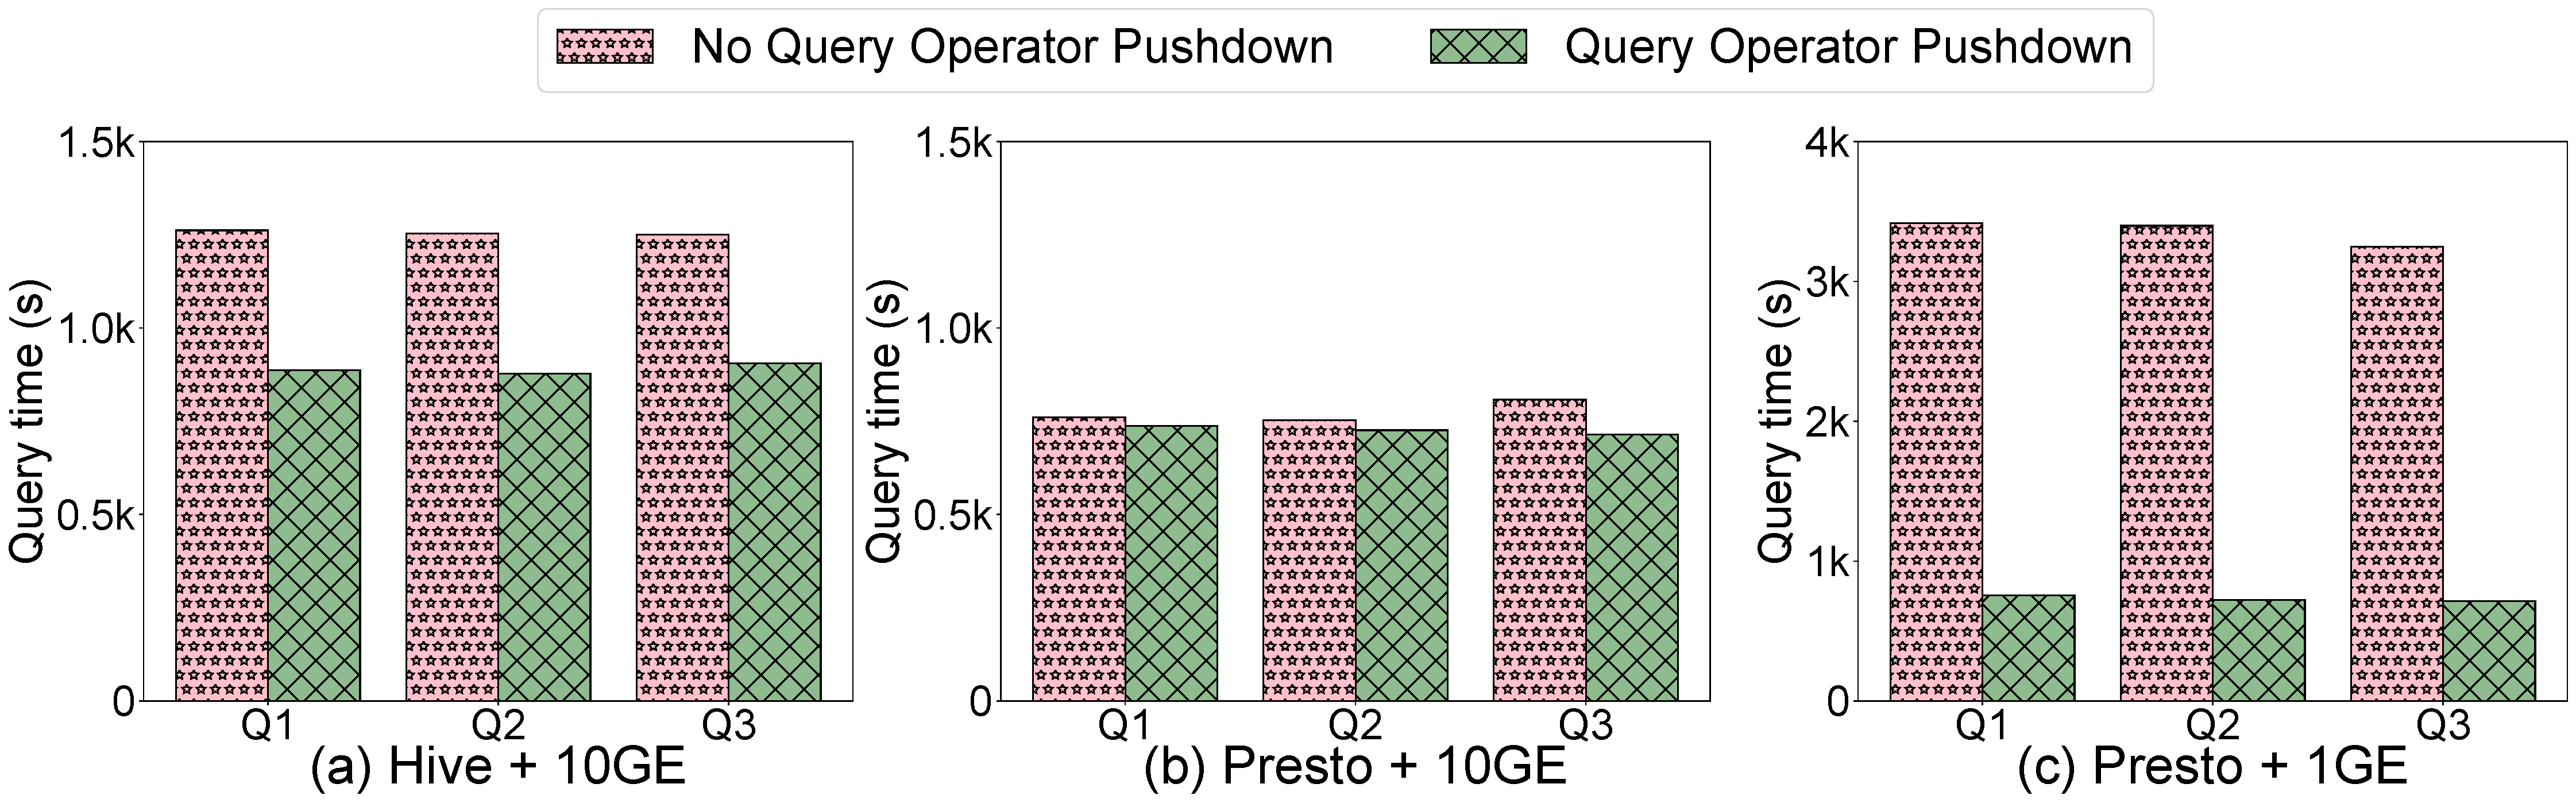
\includegraphics[width=\columnwidth]{figures/Querytime}
	\vspace{-2em}
	\caption{Computation Pushdown Query Time.}
	\label{fig:pushdown}
	\vspace{-2.1em}
\end{figure}



\subsection{Evaluation of Query Pushdown}
In this part, we evaluate the query operator pushdown  which we believe can provide stable query runtime regardless of network conditions. 
We use two groups of clusters with different network bandwidths: one with 10 GB bandwidth and the other with 1 GB. To accurately assess the benefits of the pushdown, we carefully select three live queries with data-intensive operations and 4.8 TB of data from  China Mobile. We deployed two different query engines, \texttt{Hive}~\cite{hive} and \texttt{Presto}~\cite{presto}, so as to process  SQL queries for generalization.

As shown in Figure~\ref{fig:pushdown} (the X-axis denotes the three commonly-used queries from our customers, and the Y-axis denotes the query time), 
  without query operator pushdown, query performance of baselines varies  across engines. When  queries are executed in  10 GB Ethernet, \texttt{Presto} completes the jobs in about 900 seconds, while \texttt{Hive} takes around 1200 seconds. When network bandwidth reduces to 1 GB, all execution times increase.
 In comparison, when we apply query operator pushdown, the runtime of all the queries is close to 900 seconds, regardless of compute engines and network bandwidths, which indicates a 4 times performance advantage when the engine processes queries in an 1 GB bandwidth network.  In summary, our  pushdown method introduces stable and high performance  in a storage-disaggregated architecture. 




%!TEX root = ../main.tex
\section{Related Work} 
\label{sec:related}


In this section, we will discuss relevant open-source projects and systems related to \sys $w.r.t.$ \cc{streaming platforms}, lakehouse data management, query computation pushdown and automatic database tuning.


\cc{Data lake storage system} 

%\noindent\textbf{Query computation pushdown.} NetApp~\cite{} supports Hadoop to use its storage devices through NFS-based connector docking, through S3A docking to its object storage, and through SAS/iSCSI/FC building native \hdfs on its block/lun devices. AWS EMRFS~\cite{} is an enhancement introduced to address the inconsistency of object storage in metadata operations, with official information showing that it has made computation pushdown related optimizations for the engine. Alibaba EMR is based on object storage, and the JindoFS~\cite{} solves the performance problem of object storage by introducing local data caching. These solutions improve data access to the persistent storage in computation pushdown while StreamLake offers built-in computation pushdown operations directly. 

\noindent\textbf{Streaming platforms.} Kafka, Pulsar and Pravega~\cite{} are widely-used open-source streaming platforms in industry. Unlike \sys, which builds its messaging service on top of the stream object and PLogs, and integrates its stream storage with a lakehouse framework, these solutions are file-based and require manual connections to compute engines and external storage, such as \hdfs~\cite{} or \texttt{S3}~\cite{}, for downstream processing or cost-friendly archiving. This increases both the complexity and cost of data pipeline management.



\noindent\textbf{Lakehouse.} Iceberg, Hudi and Delta Lake~\cite{} are popular  lakehouse data management framework, which rely on statistic file or object storage. 
Massive data transmission between the storage and the compute engines are inevitable in many scenarios. \cc{Not coherent!!!}
 \sys builds the lakehouse framework on top of the table object and PLogs, leveraging the enterprise-level data redundancy, high performance cache and query computation pushdown to provide reliable and high speed concurrent lakehouse reads/writes. 









%NetApp supports Hadoop by providing several connectors that enable Hadoop to use its storage devices. These connectors include an NFS-based connector for docking with NetApp's storage devices, an S3A connector for docking with NetApp's object storage, and native building of HDFS on NetApp's block/LUN devices through SAS/iSCSI/FC.

%AWS EMRFS is an enhancement introduced to address the inconsistency of object storage in metadata operations. Official information shows that AWS EMRFS has made computation pushdown related optimizations for the engine, which improve data access to persistent storage.

%Alibaba EMR is based on object storage, and it uses JindoFS to solve the performance problem of object storage by introducing local data caching. This solution improves data access to persistent storage in computation pushdown scenarios.

%StreamLake offers built-in computation pushdown operations directly, making it easy for users to take advantage of this feature without having to configure complex connectors or caching mechanisms.

%Overall, these solutions provide various ways to improve data access to persistent storage in computation pushdown scenarios, whether through native building of HDFS on block/LUN devices, improved metadata operations, or data caching.

\noindent\textbf{Automatic database tuning .} 
Recently, AI is widely-used inside the database system to improve the performance~\cite{}. For instances, OtterTune~\cite{} is a classic ML-based framework, recommending knob configuration using Gaussian process. Moreover, RL has been adopted in CDBTune~\cite{} to iteratively explore the optimal configuration.
% Investigated in [41] shows the impact of the performance variation in production environments, indicating that GP tends to converge faster but is frequently trapped in local optima, whereas RL or deep learning (DL) generally needs a longer training process and achieves better performance.
   Sun et.al~\cite{} is the first approach that tries to maximize data skipping for a partitioning using pushdown predicates with a bottom-up approach. QD-tree~\cite{} proposed a greedy algorithm and a reinforcement learning based algorithm to further optimize the partitioning strategy.
    \cc{However, these algorithms need to quantify the performance of each candidate partitioning.} %In addition, the partitioning layout is sub-optimal when new data comes, as it is optimized based on existing data.
%!TEX root = ../main.tex
\section{Conclusion} 
\label{sec:con}







%\begin{acks}
% This work was supported by the [...] Research Fund of [...] (Number [...]). Additional funding was provided by [...] and [...]. We also thank [...] for contributing [...].
%\end{acks}

%\clearpage

\bibliographystyle{ACM-Reference-Format}
\bibliography{bib/ref}

\end{document}
\endinput
